% =====================================================================
%  Multi-agent warehouse with local plan repair -- project report
%  Compile on Overleaf with pdfLaTeX (no shell-escape needed).
%  All figures live in the sub-folder  figures/.
% =====================================================================
\documentclass[10pt,a4paper]{article}

\usepackage[T1]{fontenc}
\usepackage[utf8]{inputenc}
\usepackage{lmodern}
\usepackage[margin=1in]{geometry}
\usepackage{graphicx}
\usepackage{booktabs}
\usepackage{tabularx}
\usepackage{array}
\usepackage{amsmath,amssymb}
\usepackage{xcolor}
\usepackage{caption}
\usepackage{subcaption}
\usepackage{float}
\usepackage{enumitem}
\usepackage{listings}
\usepackage{upquote}
\usepackage[hidelinks]{hyperref}

% ---------------------------------------------------------------------
%  Listings: one style for code, one for pseudocode, one for the shell.
% ---------------------------------------------------------------------
\definecolor{codegray}{gray}{0.95}
\definecolor{codekw}{RGB}{0,102,153}
\definecolor{codecm}{RGB}{90,120,90}

\lstdefinestyle{code}{
  basicstyle=\ttfamily\small,
  keywordstyle=\color{codekw}\bfseries,
  commentstyle=\color{codecm}\itshape,
  backgroundcolor=\color{codegray},
  frame=single, framerule=0.2pt, rulecolor=\color{black!40},
  columns=fullflexible, keepspaces=true, showstringspaces=false,
  breaklines=true, upquote=true, aboveskip=8pt, belowskip=8pt,
}
\lstset{style=code}

\lstdefinestyle{algo}{
  basicstyle=\ttfamily\small,
  backgroundcolor=\color{codegray},
  frame=single, framerule=0.2pt, rulecolor=\color{black!40},
  columns=fullflexible, keepspaces=true, showstringspaces=false,
  breaklines=true, upquote=true, aboveskip=8pt, belowskip=8pt,
}

\lstdefinestyle{shell}{
  basicstyle=\ttfamily\small,
  backgroundcolor=\color{black!4},
  frame=none, columns=fullflexible, keepspaces=true,
  showstringspaces=false, breaklines=true, upquote=true,
}

% Small helper: an inline code fragment.
\newcommand{\code}[1]{\texttt{#1}}

% Figure path
\graphicspath{{figures/}{./}}

\captionsetup{font=footnotesize,labelfont=bf,skip=4pt}
\setlist{nosep,leftmargin=1.4em}
% tighter vertical gaps around floats and displays
\setlength{\textfloatsep}{8pt plus 2pt minus 2pt}
\setlength{\floatsep}{6pt plus 2pt minus 2pt}
\setlength{\intextsep}{6pt plus 2pt minus 2pt}
\setlength{\abovedisplayskip}{5pt plus 2pt minus 2pt}
\setlength{\belowdisplayskip}{5pt plus 2pt minus 2pt}

% =====================================================================
\begin{document}
% ---------------------------------------------------------------------
%  Title page
% ---------------------------------------------------------------------
\begin{titlepage}
\centering

\vspace*{1.6cm}
{\Large\bfseries Multi-Robot Warehouse Operations with\par
\vspace{2pt}
Local Plan Repair\par}

\vspace{0.7cm}
{\large Partial-Order Planning, Time-Indexed Grounding and a\par
\vspace{2pt}
Negotiated Repair Protocol\par}

\vspace{0.35cm}
{\large Simulator, Protocol Design and Experimental Evaluation\par}

\vspace{2.6cm}

{\large\bfseries Submitted by\par}
\vspace{0.6cm}
\renewcommand{\arraystretch}{1.5}
\begin{tabular}{ll}
\toprule
\textbf{Name} & \textbf{Roll number}\\
\midrule
Aaditya Biswas & B23CS1001\\
Uchat Bhavya Pareshbhai & B23CS1074\\
Sanskar Patil Dhirendra & B23CS1050\\
\bottomrule
\end{tabular}

\vfill
{\large October 2026\par}
\vspace{0.6cm}
\end{titlepage}

% ---------------------------------------------------------------------
\begin{abstract}
\noindent
This report describes a discrete-time simulator, a layered planner and a
\emph{local plan-repair} engine for a fleet of warehouse robots that performs
pickup and delivery tasks on a shelf grid.  A partial-order planner (POP)
determines which actions each robot performs and in what order, a space-time
A$^\ast$ search over a time-indexed reservation table determines when and
where each robot moves, and a repair layer modifies only the robots whose
goals or path segments are invalidated by a disruption.  Repair is treated as
plan modification rather than re-planning: it does not invoke the global
planner and escalates through the rungs $R_0$--$R_4$, which bounds the scope
of any change.  When no detour without communication exists, as in the
single-door corridor used as a stress case, the affected robots
\emph{negotiate} over a short
message protocol (\textsc{Propose}, \textsc{Accept}, \textsc{Reject},
\textsc{Commit}) that grants a route through a reserved cell only if the
holder agrees and the grant accounts for the robots it alters.  In a
congested $16\times16$ warehouse with 12 robots, six
closed lanes, two breakdowns and one diversion, all 24 tasks are delivered
and every tick passes validation; the repair touches all 12 robots, but
through eight separate local passes that each take $8$--$195$\,ms of CPU.
The negotiated mode alters about one third as many robots per event as a
fleet-wide re-planning bound and is the only strategy that both remains safe
and completes the task set.  Representing the plan as a partial order keeps
downstream robots merely delayed rather than re-planned; when the ladder
fails to repair a disruption it does so by waiting, not by producing a
collision.
\end{abstract}
% =====================================================================
\section{Introduction}
% =====================================================================

A warehouse aisle is a shared resource: robots queue in it, pass each other
at its ends, and depend on each other's timing, because a tote carried by one
robot is a precondition for the next move of another.  The problem addressed
here is therefore not the routing of a single robot but the maintenance of a
consistent fleet plan while the environment changes during execution.  A
closed cross-aisle, a robot that stops working, or an urgent diversion to a
spill each invalidate part of the plan while the fleet is already executing
it.  Re-planning the whole fleet in response is neither necessary, since most
robots are unaffected, nor affordable, since it would require the fleet to
stop.

The design hypothesis examined in this report is that storing the plan as a
\emph{partial order} of robot actions, rather than as a fixed timetable,
allows a disruption to be repaired locally: the invalid part is retracted and
refined again under a least-change objective, and robots that are merely
delayed by the result are not modified.  When the local ladder cannot find a
conflict-free detour, a short negotiation between the robots holding the
contested cells supplies one.

\subsection{Problem setting and assumptions}

A fleet of $N$ robots serves pickup/delivery tasks on a two-dimensional grid
with static shelf obstacles.  A task consists of a pickup cell and a delivery
cell; each robot executes its own plan autonomously between repairs.  The
following assumptions are enforced by the simulator and by the test suite:

\begin{itemize}
  \item \textbf{Discrete space and time.}  A unit-cell grid with 4-neighbour
        moves; one robot occupies one cell per tick, and a tick is the unit of
        all scheduling decisions.
  \item \textbf{Reservations.}  A robot may use a cell or an edge only if it
        holds the corresponding time-indexed reservation (vertex, directed
        edge, or parked robot).
  \item \textbf{Bounded communication.}  A robot may negotiate only with
        robots inside a communication radius \code{comm\_radius}, and every
        repair budget (ladder depth, number of passes, candidate robots) is
        bounded.
  \item \textbf{Locality of repair.}  A repair never calls the global planner
        and never re-plans an unaffected robot: only the disrupted robot, the
        robots that must wait for it and the robots a grant actually alters
        may change.
  \item \textbf{Frozen execution.}  Steps that have started or finished are
        immutable; a repair works on the remaining suffix of the plan.
\end{itemize}
% =====================================================================
\section{System architecture}\label{sec:arch}
% =====================================================================

The implementation separates three concerns: \emph{what} has to be done and
in which order, \emph{when} and \emph{where} it happens, and \emph{how the
plan is changed} when the world changes.  This separation enables local
repair, because the repair layer can retract a single partial-order step and
let the grounding layer re-derive only the affected path segments
(Table~\ref{tab:layers}).  The planner is called \emph{once} per scenario to
produce the initial plan; subsequently the simulator invokes only the repair
engine, so a scenario run evaluates the locality of repair rather than the
quality of re-planning.

\begin{table}[H]
\centering
\small
\begin{tabularx}{\textwidth}{@{}l l X@{}}
\toprule
\textbf{Layer} & \textbf{Module} & \textbf{Responsibility} \\
\midrule
L1: partial order & \code{pocl.py} &
  STRIPS operators, threat detection and resolution, best-first POP search;
  the plan is a partially ordered set of agent actions.
\\ \addlinespace
L2: grounding & \code{planner.py}, \code{peg.py}, \code{reservation.py} &
  space-time A$^\ast$ over the time-indexed reservation table, prioritized
  grounding, plan-execution-graph retiming.
\\ \addlinespace
L3: repair & \code{modify.py}, \code{negotiation.py}, \code{metrics.py} &
  the repair phases, the $R_0$--$R_4$ escalation ladder, the message protocol
  and the altered-agent metrics.
\\
\bottomrule
\end{tabularx}
\caption{The three layers and the modules that implement them.  Around them
sit the instance model (\code{world.py}, \code{scenarios.py}), the event
generator (\code{disruptions.py}), the tick loop and validator
(\code{sim.py}), the visualisations (\code{viz.py}, \code{viz\_plan.py}), the
ablation baselines (\code{baselines.py}) and the sweeps
(\code{experiments.py}).}
\label{tab:layers}
\end{table}

The repair layer is integrated into the planner rather than applied after it,
so the data flow is linear with a single feedback edge:

\begin{lstlisting}[style=shell]
world.py -> pocl.py -> peg.py -> planner.py -> sim.py -> viz.py / viz_plan.py
             |                                 ^
             +-- repair: modify.py -------------+-- negotiation.py   (R0..R4)
                                |
                          disruptions.py / metrics.py
\end{lstlisting}

\begin{table}[H]
\centering
\small
\begin{tabularx}{\textwidth}{@{}l X@{}}
\toprule
\textbf{Pipeline element} & \textbf{Warehouse meaning} \\
\midrule
action & \code{Goto} / \code{Pick} / \code{Drop} (L1) and \code{Move} / \code{Act} (L2, L3)\\
causal link & \code{at}, \code{holding}, \code{hand\_empty} (L1); a cell hand-over \code{Free(cell)} (L3)\\
ordering constraint & a precedence edge between two steps\\
threat & a new visit inside another robot's hand-over slot on the same cell\\
threat resolution & promotion/demotion, i.e.\ \emph{who waits for whom}\\
open condition & unsupported precondition (\code{operational(a)}, \code{delivered(o)})\\
exogenous step & \code{Block}/\code{Unblock} and \code{Break}/\code{Fix}\\
plan reuse & repair starts from the existing plan instead of a fresh search\\
\bottomrule
\end{tabularx}
\caption{Classical partial-order planning vocabulary in warehouse terms.}
\label{tab:mapping}
\end{table}
% =====================================================================
\section{Layer 1: partial-order planning}\label{sec:pocl}
% =====================================================================

Each robot receives its own partial-order plan (POP).  Planning per robot
keeps the set of ground actions small, since cross-robot constraints are
introduced later as reservations (Section~\ref{sec:ground}), and it is also
what makes a repair local, because a disruption only removes or reorders
steps of the plans it affects.

\subsection{STRIPS domain}

Facts are tuples, for example $(\text{at},a,\ell)$ (\emph{robot $a$ is at
cell $\ell$}), $(\text{holding},a,o)$ and $(\text{hand\_empty},a)$.  The
operator library is small and fixed.

\begin{table}[H]
\centering
\small
\setlength{\tabcolsep}{4pt}
\begin{tabularx}{\textwidth}{@{}l X X X c@{}}
\toprule
\textbf{Action} & \textbf{Preconditions} & \textbf{Add} & \textbf{Delete} & \textbf{Duration}\\
\midrule
\code{Goto(a,x,y)} & \code{at(a,x)}, \code{operational(a)} & \code{at(a,y)} & \code{at(a,x)} & BFS dist.\\
\code{Pick(a,o,l)} & \code{at(a,l)}, \code{at\_item(o,l)}, \code{hand\_empty(a)} & \code{holding(a,o)} & \code{hand\_empty(a)}, \code{at\_item(o,l)} & 1\\
\code{Drop(a,o,l)} & \code{at(a,l)}, \code{holding(a,o)} & \code{delivered(o)}, \code{hand\_empty(a)} & \code{holding(a,o)} & 1\\
\code{Emergency(a,E)} & \code{at(a,E)}, \code{operational(a)} & \code{emergency\_done(a)} & --- & hold time\\
\bottomrule
\end{tabularx}
\caption{The STRIPS operator library.  Ground actions are instantiated only
over the locations that matter for the robot (roughly $2\cdot\text{tasks}+2$
cells), which keeps the branching factor small.}
\label{tab:strips}
\end{table}

\subsection{Search}

The search is best-first over partial plans.  At each step one \emph{flaw} is
selected, first among threats and then among open conditions with the fewest
achievers, and is refined either by \emph{reuse} (an action already present
in the plan achieves it) or by inserting a new action from the library.  A
threat is resolved by \emph{promotion} or \emph{demotion}, that is, by adding
an ordering constraint.  The ranking function is
%
\[
  f(P) \;=\; g(P) + \bigl|\text{open}(P)\bigr|,
  \qquad
  g(P) \;=\; \sum_{\text{Goto}} \text{duration} \;+\; \#\{\text{non-Goto steps}\},
\]
%
so the search favours plans with low travel cost and few actions, with the
number of remaining flaws used as a tie-breaker in favour of plans closer to
completion.

\subsection{Validity and soundness}

A candidate plan is accepted only if \code{is\_valid\_pop} holds: every
precondition of every step is supported by a causal link, no threat remains
between a link and an interfering step, and the ordering graph is acyclic.
Validity is additionally checked by execution: the plan is sampled twenty
times at random topological orders, each order is executed in STRIPS style
from the initial state, and every sample must reach all goals.  This detects
orders that satisfy the constraint graph but violate the operator semantics,
and it is inexpensive enough to run inside the search loop.  A plan that is
valid for a single robot is therefore complete for that robot's own goals;
cross-robot constraints are introduced afterwards as reservations.
\begin{figure}[H]
\centering
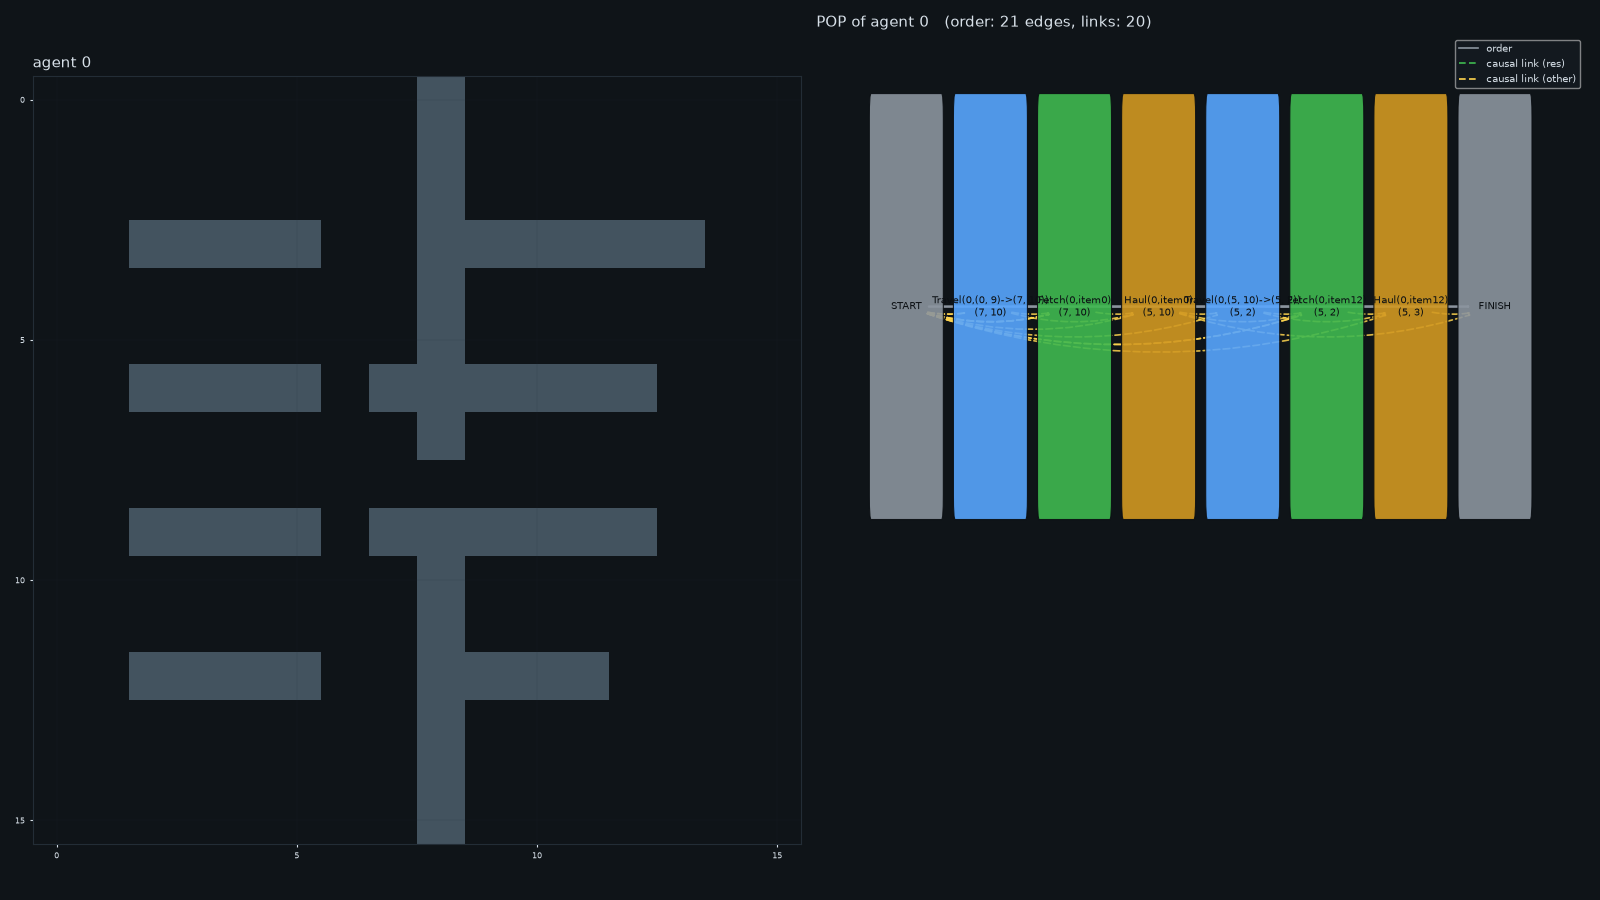
\includegraphics[width=0.72\textwidth]{caseA_pop.png}
\caption{A partial-order plan of one of the robots that the repair altered in
case study~A.  Solid edges are ordering constraints, dashed edges are causal
links (\code{at}, \code{holding}, \code{hand\_empty}); the layered layout is
the topological depth.  Because the plan is a partial order, a delay only
shifts the steps of the affected chain and does not require a new plan.}
\label{fig:pop}
\end{figure}

% =====================================================================
\section{Layer 2: time-indexed grounding}\label{sec:ground}
% =====================================================================

Grounding converts the partial order into a collision-free schedule.  The
shared resource is the \emph{reservation table}, a set of time-indexed
reservations over \textbf{vertices} (robot $a$ occupies cell $c$ at tick
$t$), \textbf{directed edges} (robot $a$ traverses $c \to c'$ between $t$ and
$t+1$; the reverse edge is a distinct reservation, which makes swaps
detectable) and \textbf{parks} (an idle robot keeps its cell reserved until it
moves).  A \emph{clash} is an attempt to reserve a vertex, edge or park that
another robot already holds.  Paths are found by space-time A$^\ast$ over the
graph of $(\text{cell}, \text{tick})$ states with the Manhattan distance as an
admissible heuristic, in one of two modes: \textbf{hard}, in which clashed
states are forbidden and a segment with fixed endpoints must not disturb any
other robot (the self-reroute of $R_1$), and \textbf{soft}, in which a clash
is permitted but priced by \code{lambda\_soft}, used when a robot needs only
to determine which cells and which robots it would have to negotiate with.

The initial plan is produced by \emph{prioritized grounding}: robots are
ordered by priority (an emergency robot first, then the robot with the lower
id), and each is planned by hard space-time A$^\ast$ against the reservations
of the robots already committed.  Because every reservation is time-indexed,
mutual waiting is representable: a robot that finds a door occupied waits one
tick and retries, which is the behaviour required in a congested aisle.

\subsection{The plan-execution graph (PEG)}

The grounded plan is stored as a plan-execution graph.  Nodes are micro-steps
with never-reused identifiers and a pointer to the partial-order step they
realise; edges carry the timing constraint and come in three kinds: \code{seq}
(consecutive micro-steps of one robot, weight equal to the duration of the
source step), \code{logic} (the \code{Pick} that makes a tote available to the
matching \code{Drop}) and \code{res} (a resource edge of weight \textbf{0},
added start-to-start between consecutive visitors of a cell).

For every cell $c$ the graph keeps the occupancy sequence
$\mathrm{occ}[c] = [(a_i, \text{enter}_i, \text{leave}_i)]$ sorted by
arrival, and for two consecutive visits by different robots it adds the
weight-0 edge $\text{leave}_p \to \text{enter}_q$, so that a robot may
\emph{follow} another into a cell on the tick it is vacated.  These edges
also allow collisions to be detected on the graph rather than on the
schedule: a vertex swap, a head-on conflict and a rotation conflict all
appear as a cycle in the PEG, so \code{peg.is\_acyclic()} is a complete
collision-safety check, because any assignment of times that respects every
edge is free of vertex and swap collisions.  This reduces an expensive
pairwise schedule check to a single topological test, which is inexpensive
enough to run inside every tentative repair candidate, including the deep
copies used during negotiation.
\subsection{Retiming and validation}

\code{retime(peg, t\_now)} recomputes the schedule of a possibly patched
graph: steps that have already started or finished keep their actual times,
and every other step is scheduled in topological order by
%
\[
  s.t \;=\; \max\Bigl(\{t_{\text{now}}\} \cup \{s.\text{anchor}\} \cup
  \{\,p.t + w(p,s) \;:\; p \in \text{preds}(s)\,\}\Bigr),
\]
%
where the anchor is used only when it is not \code{None}.  A patched plan
therefore does not have to be re-grounded from scratch, only re-timed, which
keeps a repair inexpensive.

The simulator validates every tick of every run in every mode: a vertex
clash, a swap, a move into a shelf, a move into a blocked cell and a
collision with a parked robot are all violations, and the graph must
additionally be acyclic.  A repair that would produce a violation is aborted
and rolled back to the previous plan.  Validation is recorded per run and
reported in every comparison below; it is the result that exposes the global
re-planning bound in Section~\ref{sec:experiments}.

\begin{figure}[H]
\centering
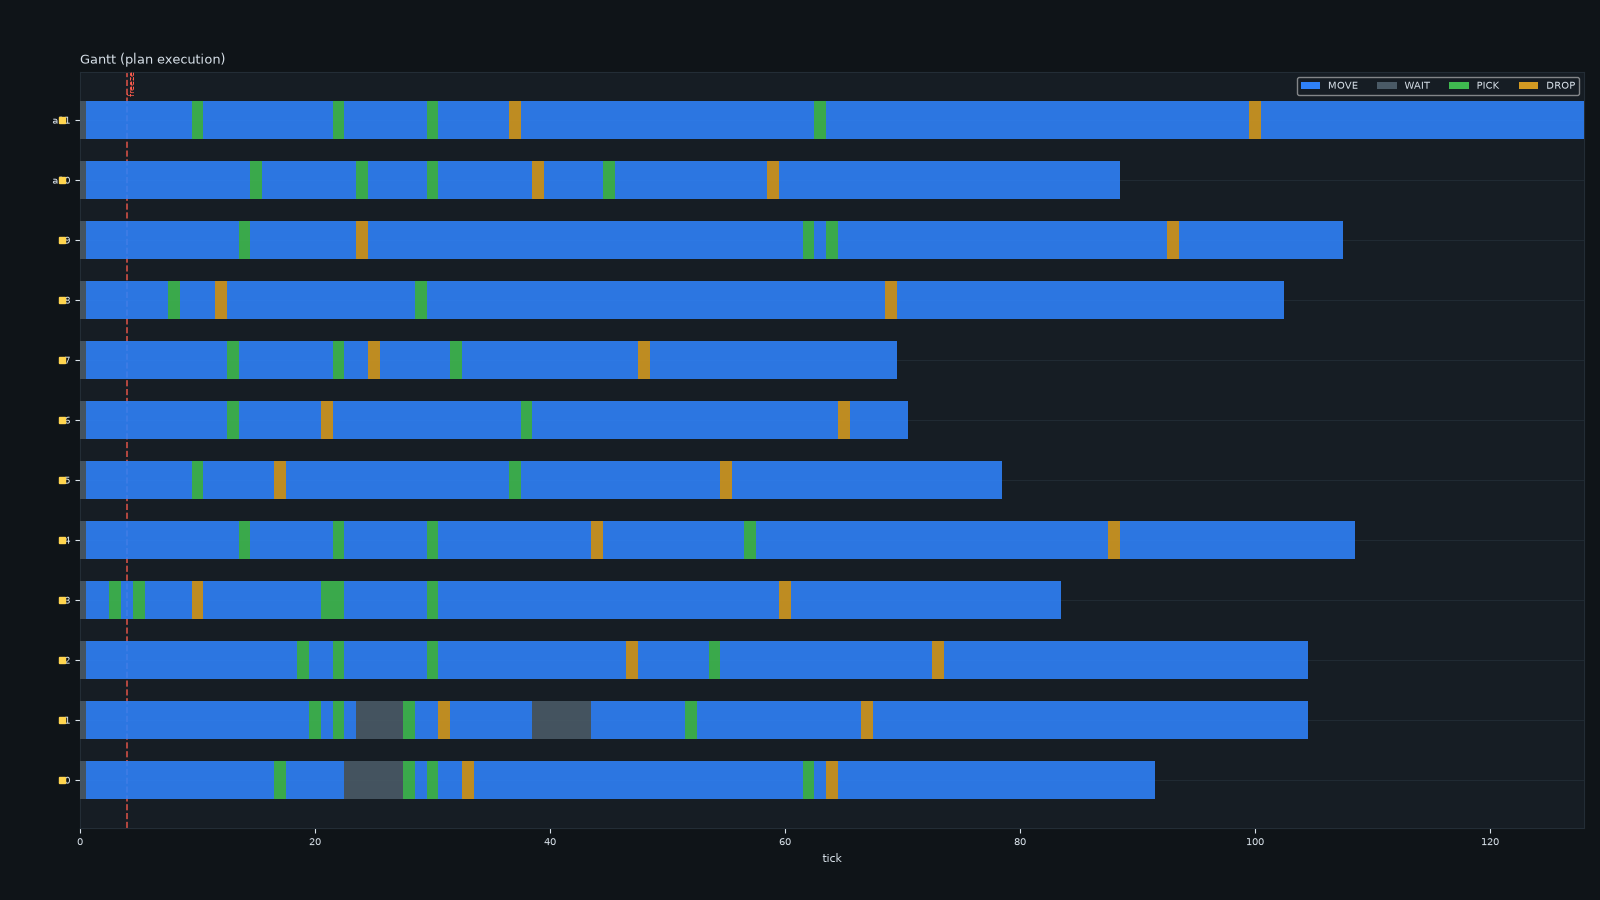
\includegraphics[width=0.84\textwidth]{caseA_gantt.png}
\caption{Per-robot Gantt chart of the repaired schedule of case study~A.
Rows are robots, columns are ticks, and the colour is the robot's altered
category, so the yellow and orange rows are the robots that the ladder
modified, while the grey rows only shifted in time.}
\label{fig:gantt}
\end{figure}

% =====================================================================
\section{Disruptions as plan flaws}\label{sec:disruptions}
% =====================================================================

A disruption is modelled not as an exception that interrupts a plan but as
\emph{exogenous steps inserted into the plan}, which leave the plan in an
invalid state.  The repair engine therefore receives a plan with flaws, in
the same form as the planner.  All events of a scenario are derived from the
\emph{undisrupted} plan before any repair occurs, so every strategy receives
the identical event list and comparisons between strategies differ in a
single variable.

\begin{table}[H]
\centering
\small
\begin{tabularx}{\textwidth}{@{}l l X@{}}
\toprule
\textbf{Event} & \textbf{Exogenous steps} & \textbf{Resulting flaws}\\
\midrule
Cell blockage & \code{Block(c)} at $t$, \code{Unblock(c)} at $t\!+\!D$ &
  later visits of $c$ must be ordered after \code{Unblock} (demotion $=$
  wait); if waiting costs more than the threshold, the leg is rerouted.\\
Breakdown & \code{Break(a)} at $t$, \code{Fix(a)} at $t\!+\!D$, \code{Fix}
  $\to$ next step of $a$ &
  \code{operational(a)} is violated for $D$ ticks; followers wait through
  \code{res} edges; a robot whose delay exceeds the threshold reroutes.\\
Permanent breakdown & \code{Break(a)} only &
  the remaining goals of $a$ become orphans (and \code{at\_item(o,cell)} if a
  tote is carried); visits to $a$'s cell must be rerouted.\\
Emergency & \code{Emergency(a,E)} before the remaining steps &
  an open condition \code{emergency\_done(a)} plus \code{at(a,E)}: the
  planner inserts the detour and restores the original \code{at} link.\\
\bottomrule
\end{tabularx}
\caption{Every disruption class reduced to exogenous plan steps and the flaws
those steps create.}
\label{tab:events}
\end{table}

The simulator replays the events in \textbf{tick order} under three rules: a
repair pass sees only the events announced at or before its tick, so a later
blockage cannot justify an earlier decision; a blockage is \emph{postponed}
while it would trap a robot inside an already-executed step; and an accident
hold is a \emph{constraint on the new plan} and is never introduced into the
frozen prefix.  Residual safety violations are checked per time window, so a
plan that is consistent at each tick cannot accumulate into an inconsistent
schedule.
% =====================================================================
\section{Local plan repair}\label{sec:repair}
% =====================================================================

A repair is a \emph{plan modification} in the style of
Kambhampati--Hendler: retract only the invalid parts, then refine with a
least-change search, in four phases.

\begin{enumerate}
  \item \textbf{Diagnose.}  Copy the PEG, insert the exogenous steps, retime,
        and compute the affected set $A_0$ together with the flaw list:
        threatened resource links, unsupported preconditions, unreachable
        legs and orphan goals.
  \item \textbf{Unrefine.}  Retract \emph{only} what is invalid.  A threat
        that an ordering constraint can resolve retracts nothing; a leg
        through a blocked cell retracts that leg's unstarted micro-steps; a
        permanent breakdown retracts the robot's unstarted steps.  Started
        and finished steps are never touched: the executed prefix is
        re-rooted as the new start of the plan.
  \item \textbf{Refine and negotiate.}  Escalate through the ladder
        $R_0$--$R_4$ below, stopping at the first acceptable candidate
        (Figure~\ref{fig:phases} shows the phases of the deepest pass).
  \item \textbf{Commit.}  Two-phase: assert acyclicity, run the simulator
        validator, otherwise abort and roll back to the previous plan.
\end{enumerate}

\begin{table}[H]
\centering
\small
\setlength{\tabcolsep}{5pt}
\begin{tabularx}{\textwidth}{@{}l X X@{}}
\toprule
\textbf{Rung} & \textbf{Operation} & \textbf{Who may change}\\
\midrule
$R_0$ & retime only (the new ordering edges \emph{are} the waiting) &
  robots that gain an incoming edge\\
$R_1$ & self-reroute of the affected \code{Goto} leg with \emph{hard}
  space-time A$^\ast$ (fixed endpoints), then insert the visit &
  the robot itself, plus the robots that now wait\\
$R_2$ & negotiation (Section~\ref{sec:negotiate}) within \code{comm\_radius},
  depth $\le$ \code{max\_depth} & the negotiation chain\\
$R_3$ & $R_2$ with \code{comm\_radius} $+\;3$ (at most twice) &
  the same, with a wider audience\\
$R_4$ & reassignment of orphan goals via POCL from the receiver's own plan &
  the broken robot and the receivers\\
fallback & keep $R_0$ (the robots wait), retry each tick; after
  \code{failure\_wait} ticks record \code{success = False} & ---\\
\bottomrule
\end{tabularx}
\caption{The escalation ladder.  The global planner is never called; the
worst case, in which every robot waits, preserves correctness rather than
losing locality.}
\label{tab:ladder}
\end{table}

Two acceptance rules govern the ladder.  A candidate is \emph{acceptable}
only if its total added delay does not exceed \code{delay\_threshold}, and
candidates are \emph{ranked} by a least-change cost
%
\[
  \text{cost}(c) \;=\; \text{added\_delay\_total}(c) \;+\;
  \beta_{\text{alter}} \cdot \bigl|\text{altered\_plan}(c)\bigr| ,
\]
%
so that a detour that is slightly longer but affects fewer robots is
preferred.  The weight $\beta_{\text{alter}}$ prices one altered robot in
units of delay; the lexicographic rule of the specification is the limit
$\beta_{\text{alter}} \to \infty$ of this cost.
\subsection{The negotiation protocol}\label{sec:negotiate}

Waiting is available at no cost and requires no communication, but a detour
that needs a cell another robot holds as a \emph{park} cannot be taken
unilaterally.  The protocol addresses this case: the repair requests
permission from the \emph{holder} of the contested cell, and the holder
decides according to whether the request is acceptable in terms of the robots
it alters.

\begin{lstlisting}[style=algo]
negotiate(i, depth, chain):
    path, C <- st_astar_soft(i, reservations)      # C = clashed holders
    if C is empty:
        apply path to a COPY of the PEG; return SUCCESS
    for j in C, in order of promise:
        if dist(i, j) > comm_radius or j in chain: continue
        PROPOSE_ORDER(i -> j, visit, link, before | after)
        j answers:
            1. grant is acyclic and delay(j) <= 2*delay_threshold -> ACCEPT(delay)
            2. else j reroutes its own leg, everybody else frozen -> ACCEPT(delay)
            3. else if depth < max_depth -> sub-negotiate, ACCEPT / REJECT
            4. else REJECT(reason)
    if every holder ACCEPTed:
        COMMIT; assert the patched PEG is acyclic -> SUCCESS
    else:
        ABORT; add every rejected clash as a HARD constraint; retry <= 3
\end{lstlisting}
Five properties of the protocol keep the repair local.
\textbf{The proposal is a complete route, not a cell}: the initiator computes
its remaining route in \emph{soft} mode and collects the set $C$ of holders
it clashed with, so a negotiation concerns a concrete route and a
\textsc{Reject} answer is specific.  \textbf{Acceptance by waiting has no
cost}: robots re-planned after the initiator are re-derived against the
initiator's new reservations and simply wait or reroute, requiring no further
message, so most negotiations alter very few robots.  \textbf{A
grant must be beneficial}: the initiator accepts only when its own saving
exceeds both the delay threshold and the $\beta_{\text{alter}}$ price of
every robot that the grant newly alters, and a granted route is then verified
clash-free against every non-yielding holder, so a grant cannot introduce a
collision.  \textbf{Rejection is explicit}: a holder rejects if it is
physically held (accident, breakdown or emergency hold), if its plan is
frozen (outside the replan set, or already committed earlier in the same
pass) or if the chain would close a cycle; the rejected clash remains a hard
constraint for the initiator, which then falls back to the hard space-time
A$^\ast$ regrounding of the ladder.  \textbf{Widening rather than escalation
to the global planner}: a holder that is outside \code{comm\_radius} but
inside $\code{comm\_radius} + 3\,(\code{max\_depth}-\text{depth})$ is added
to the replan set, which is rung $R_3$.

Every message (\textsc{Propose\_Order}, \textsc{Propose\_Reroute},
\textsc{Accept}, \textsc{Reject}, \textsc{Commit}, \textsc{Abort}) is
recorded, counted by type and exported into the repair record, the simulator
trace and the message arrows of the visualisation; the panel counter
\emph{protocol messages} can therefore be read directly from a run.

\begin{figure}[H]
\centering
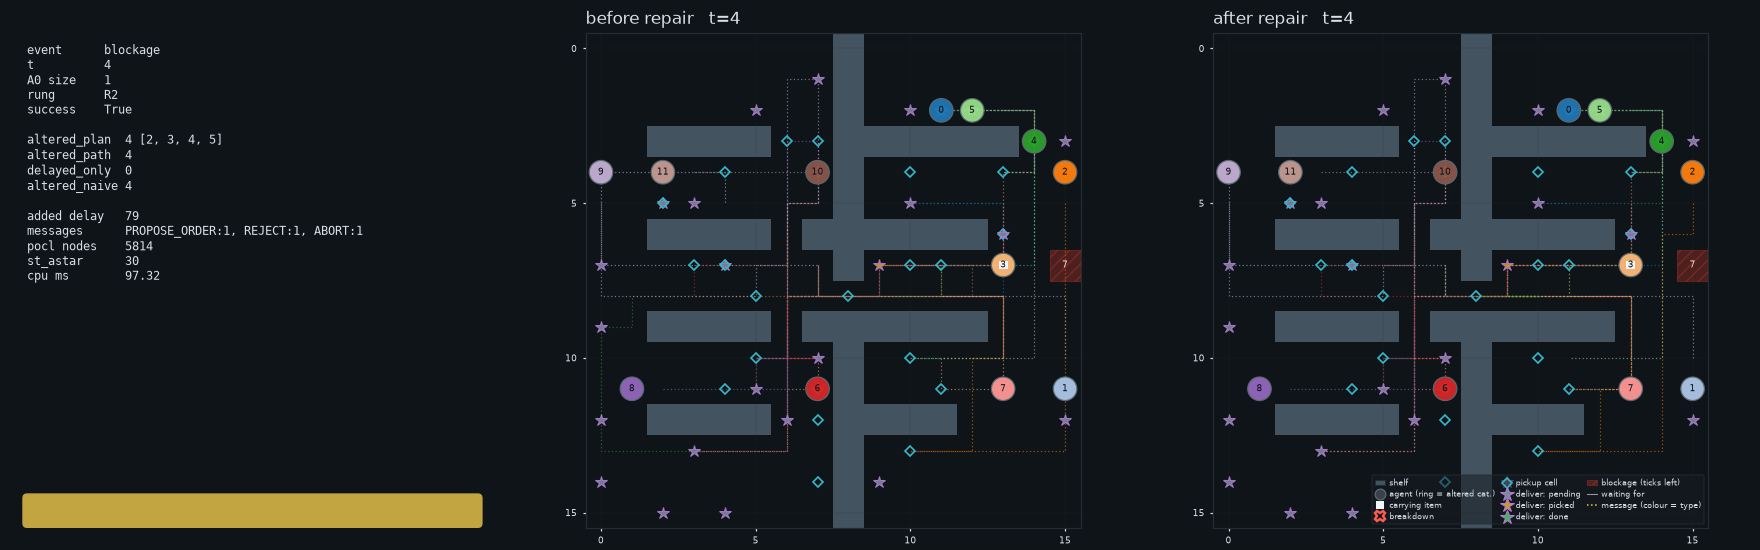
\includegraphics[width=0.90\textwidth]{caseA_repair_card_00.png}\par\vspace{3pt}
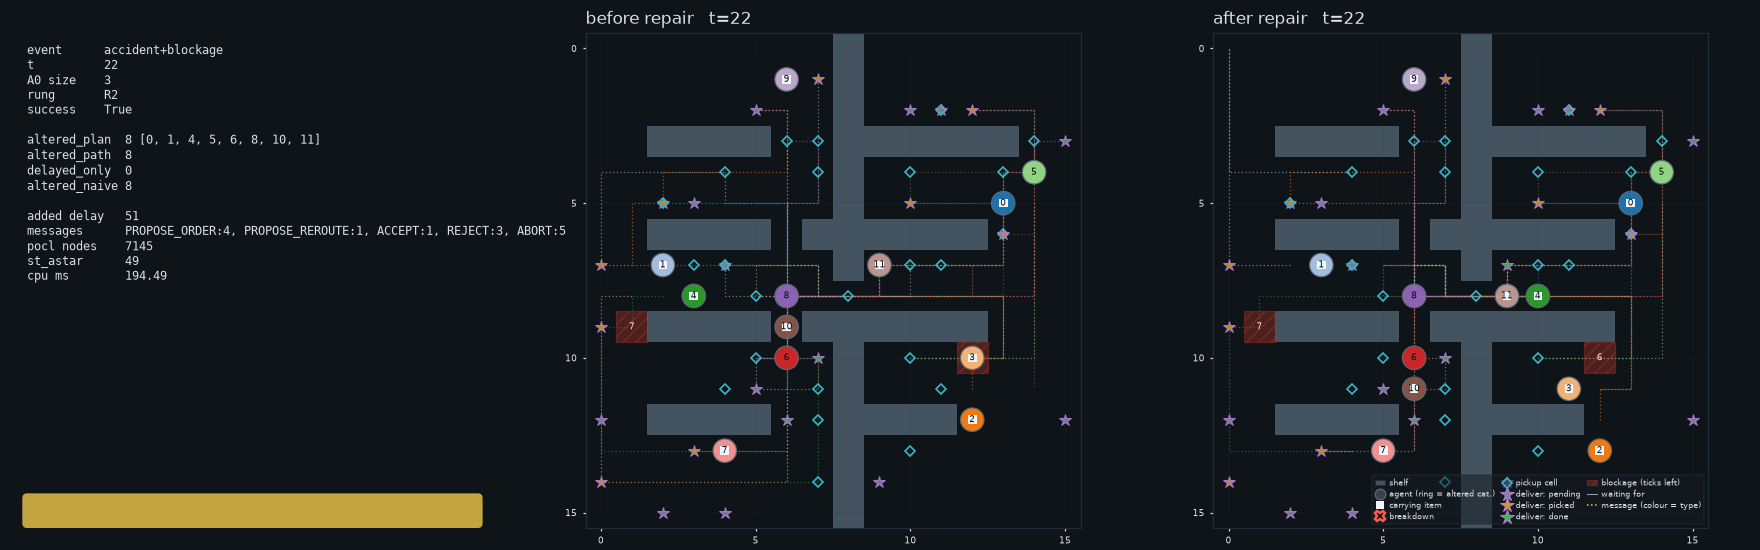
\includegraphics[width=0.90\textwidth]{caseA_repair_card_02.png}
\caption{Two of the four repair cards of case study~A (the artefacts contain
the cards of all eight passes): the first lane closure ($t=4$) and the
accident ($t=22$), the deepest pass of the shift.  A card is the printed form
of one \code{RepairRecord}: rung, the four altered sets, the message counts
and the budgets on the left, and the before/after routes on the right.  Every
claim of a row of Table~\ref{tab:passesA} is visible on the corresponding
card.}
\label{fig:cards}
\end{figure}

\begin{figure}[H]
\centering
\begin{subfigure}[t]{0.47\textwidth}
  \centering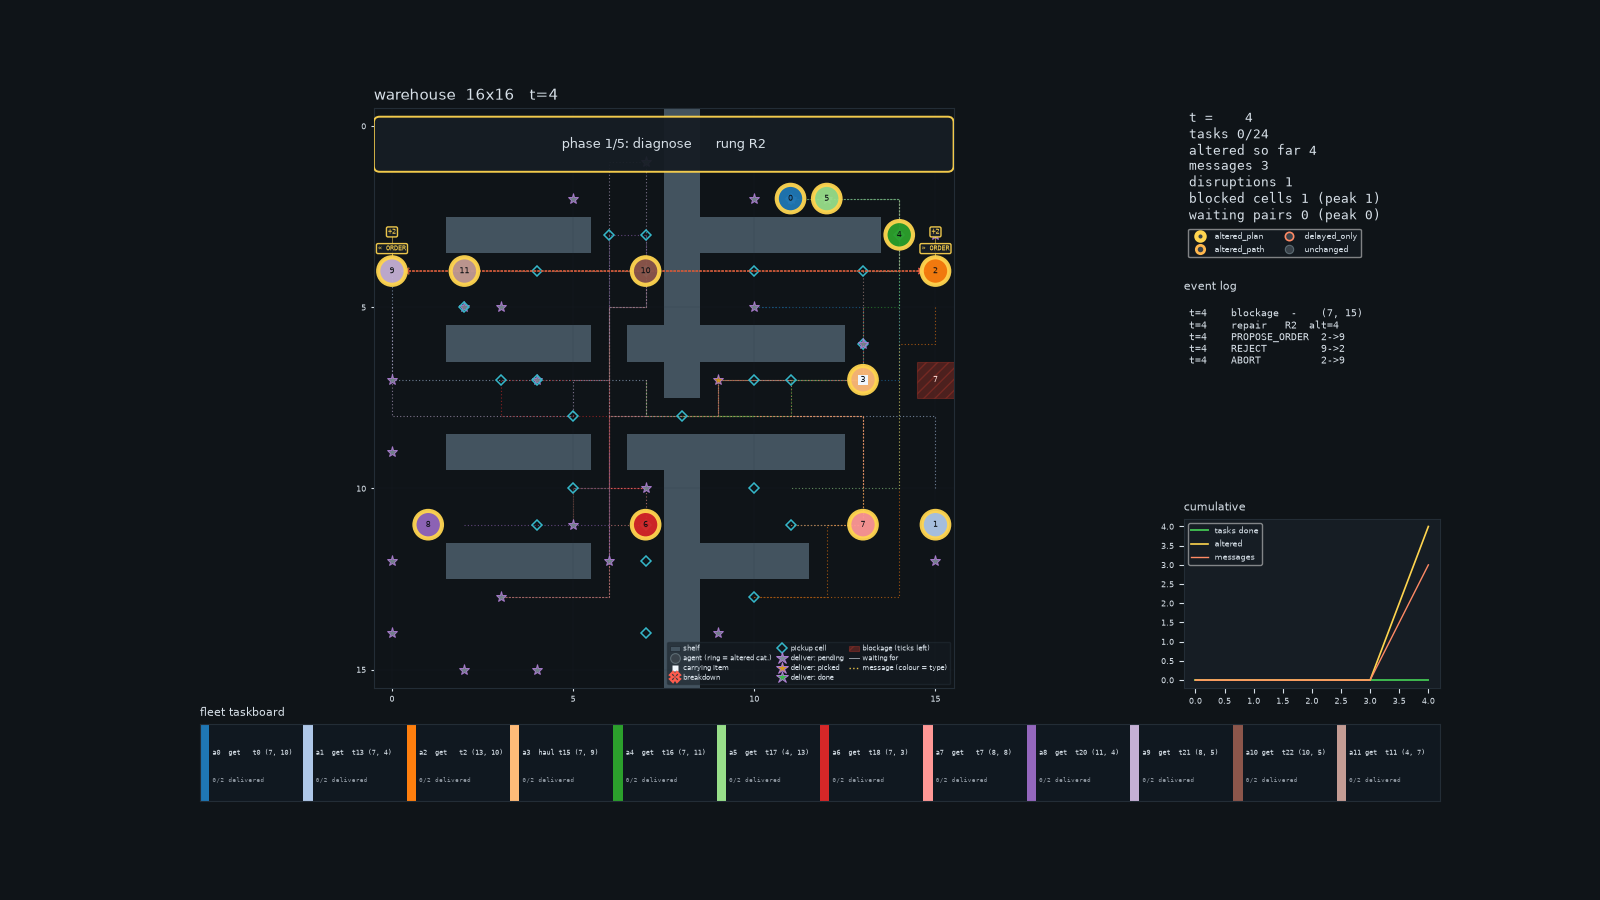
\includegraphics[width=\linewidth]{caseA_phase_diagnose.png}
  \caption{phase 1: diagnose ($A_0$ and the flaws)}
\end{subfigure}\hfill
\begin{subfigure}[t]{0.47\textwidth}
  \centering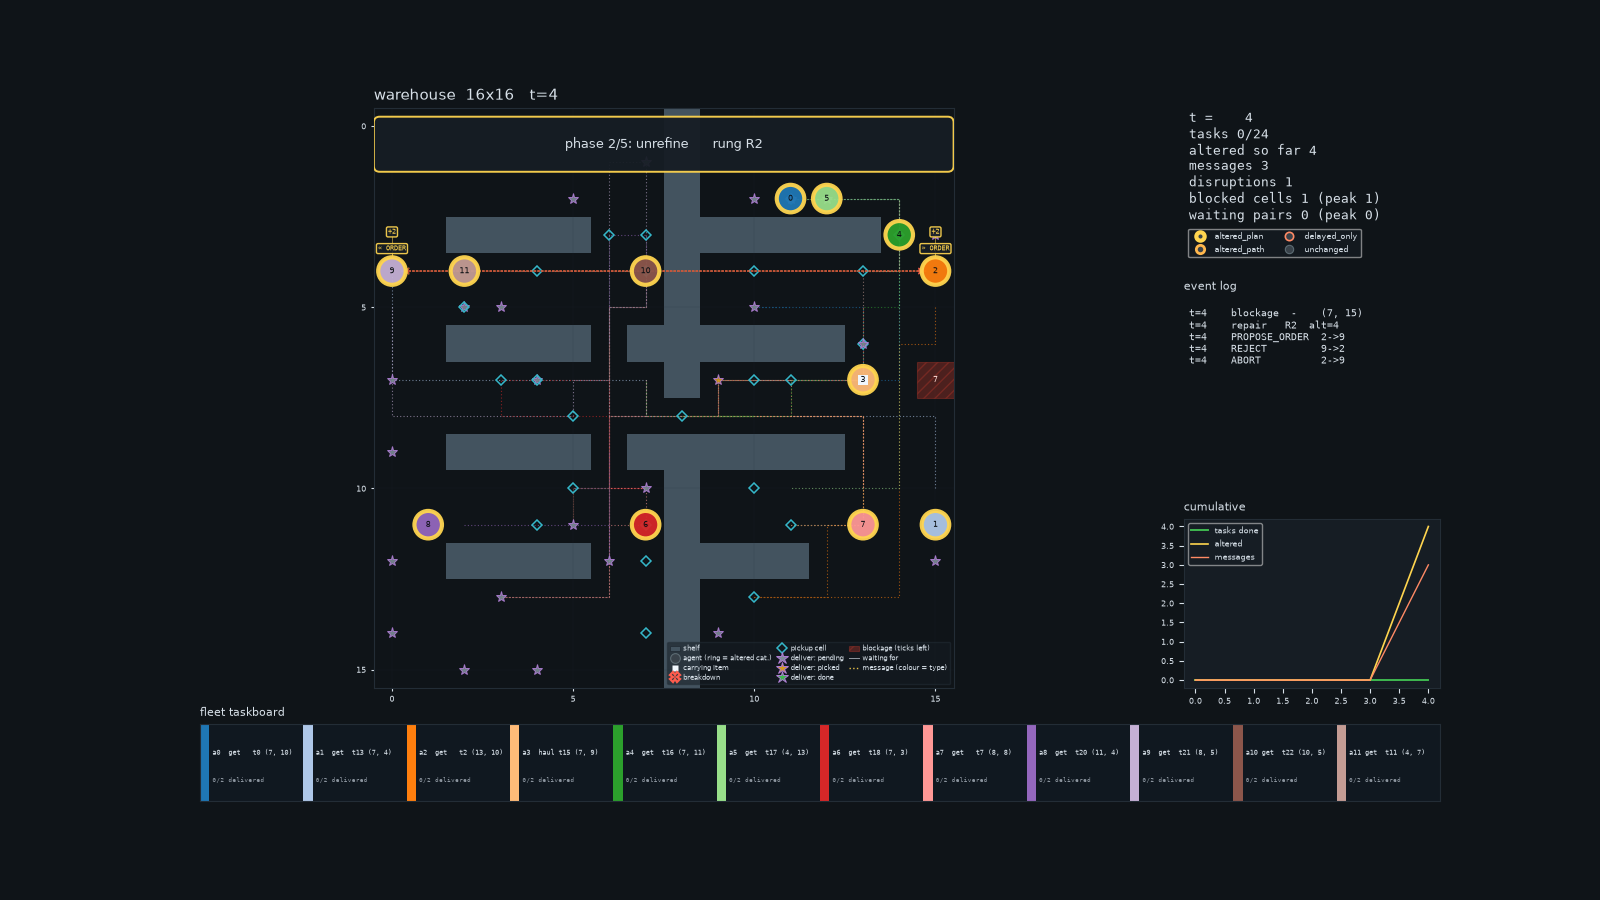
\includegraphics[width=\linewidth]{caseA_phase_unrefine.png}
  \caption{phase 2: unrefine (retract what is invalid)}
\end{subfigure}

\vspace{4pt}
\begin{subfigure}[t]{0.47\textwidth}
  \centering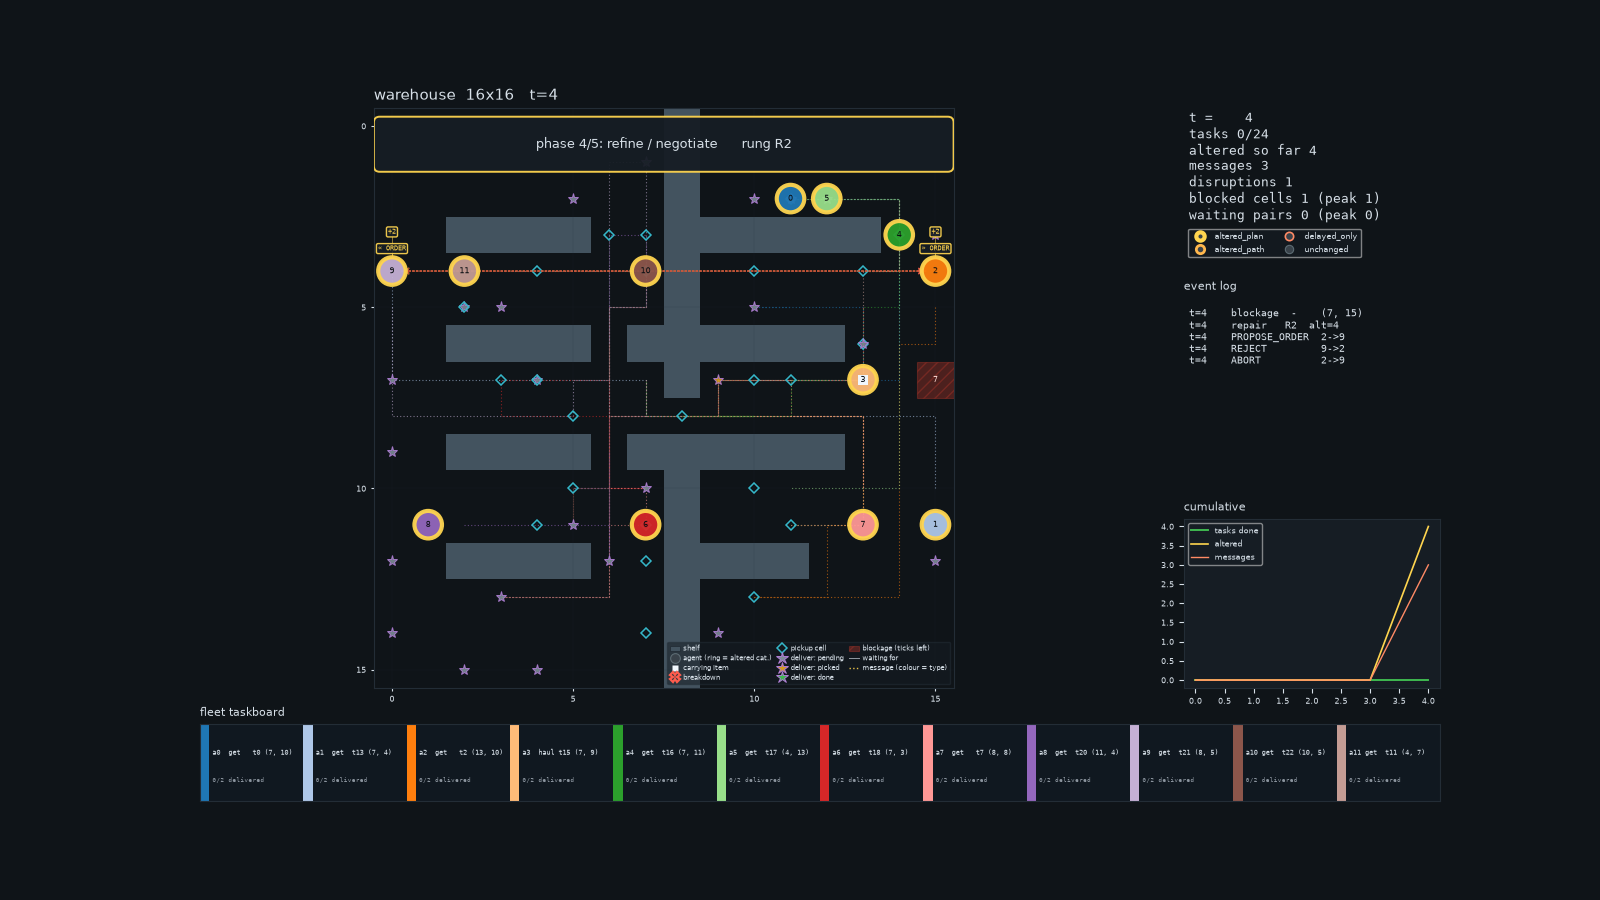
\includegraphics[width=\linewidth]{caseA_phase_negotiate.png}
  \caption{phase 3: refine / negotiate (ask the holders)}
\end{subfigure}\hfill
\begin{subfigure}[t]{0.47\textwidth}
  \centering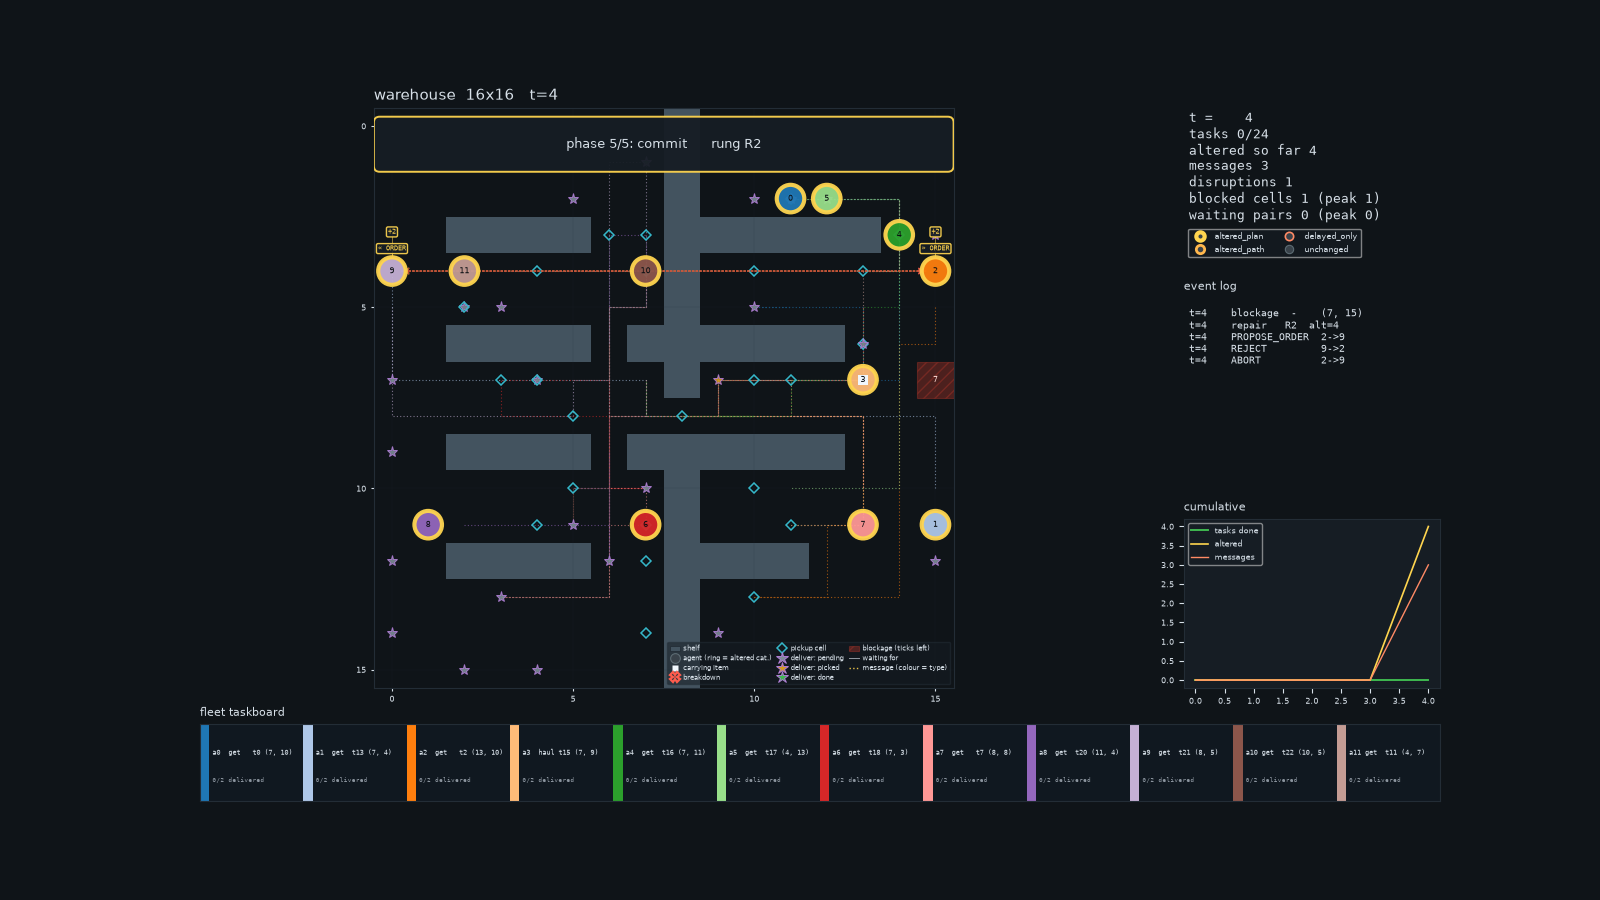
\includegraphics[width=\linewidth]{caseA_phase_commit.png}
  \caption{phase 4: commit (acyclicity and the validator)}
\end{subfigure}
\caption{The phases of the deepest pass of case study~A (the accident at
$t=22$, resolved at rung $R_2$), each drawn on the freeze tick.  The
escalation is visible in the banner: $R_1$ is attempted first and is not
sufficient here, so the pass ends at $R_2$.}
\label{fig:phases}
\end{figure}
% =====================================================================
\section{Measuring what a repair changed}\label{sec:metrics}
% =====================================================================

The question of how local the repair is requires a precise definition of
``changed''.  Four nested measures of the same event are therefore reported,
all computed on the \emph{remaining} plan, that is, on the steps strictly
after the freeze tick, so that edits to the already-executed prefix cannot
inflate the assessment of a repair.

\begin{table}[H]
\centering
\small
\begin{tabularx}{\textwidth}{@{}l l X@{}}
\toprule
\textbf{Metric} & \textbf{Signature compared} & \textbf{Meaning}\\
\midrule
\code{altered\_plan} \emph{(primary)} & action sequence and its content &
  the robot's \emph{plan} really changed: a new step, a lost step, a
  different action or a new ordering.\\
\code{altered\_path} & run-length-encoded cell route &
  the \emph{route} changed: a new cell is visited (or a task is reassigned).
  Inserting a wait never changes this signature.\\
\code{delayed\_only} & route identical, times different &
  the robot only waits: the cheapest and most desirable outcome of a
  repair.\\
\code{altered\_naive} & any differing $(\text{cell}, t)$ pair &
  the naive diff-the-trace definition; it counts a pure time shift as a
  change, and therefore upper-bounds the other three.\\
\bottomrule
\end{tabularx}
\caption{The four altered-agent definitions, ordered by severity.  A repair
that produces only \code{delayed\_only} robots has not re-planned any robot.}
\label{tab:altered}
\end{table}

A repair pass also produces one \code{RepairRecord} per event: event type,
tick, $|A_0|$, resolved rung, the four altered id sets,
\code{added\_delay\_total}, \code{messages\_by\_type}, POP nodes, ST-A$^\ast$
calls, \code{cpu\_ms} and \code{success}.  The record provides the fields
printed on a repair card and aggregated by the sweeps.

As an example, at $t=29$ a lane closes and the pass is resolved at rung
$R_1$ by a pure self-reroute, with \code{altered\_plan} $=7$ while
\code{altered\_path} and \code{altered\_naive} are $8$.  The eighth robot has
an unchanged route and only a change in timing, so the plan measure excludes
it while a naive trace difference counts it.  The largest pass is the $t=22$
accident, with $A_0=8$, resolved at $R_2$ after three negotiated passes,
ending with $17$ cumulative protocol messages and $51$ ticks of added delay.
Aggregated over the eight passes, \code{altered\_plan} has mean $4.00$,
median $3$ and maximum $8$; \code{altered\_path} and \code{altered\_naive}
have mean $4.125$; and \code{delayed\_only} is $0.00$, indicating that in a
warehouse of this density every delay large enough to be repaired also
introduces a new cell or ordering.
% =====================================================================
\section{Experiments}\label{sec:experiments}
% =====================================================================

\subsection{Setup}

All results were produced on one machine with Python 3.12, NumPy, pandas and
Matplotlib, in a single deterministic configuration.  Every run is
seed-controlled, and the only non-reproducible column of any table is the
wall-clock \code{cpu\_ms} of a repair pass.  Three instance families are
used, and the event generator is independent of the repair strategy: the
event list is derived once from the undisrupted plan and replayed for every
mode, so a comparison across modes varies one variable only.

\begin{table}[H]
\centering
\small
\begin{tabularx}{\textwidth}{@{}l X c c X@{}}
\toprule
\textbf{Instance} & \textbf{Grid} & \textbf{Robots} & \textbf{Tasks} & \textbf{Disruptions}\\
\midrule
A: congested shift & $16\times16$, 49 shelves, one cross-aisle walled off
  (single door at $(8,8)$) & 12 & 24 & 6 closed lanes, 2 breakdowns,
  1 emergency ($=$ 9 events)\\
B: corridor choke point & $8\times10$, wall at column 3, single door at
  $(3,3)$ & 4 & 3 & 2 accidents (the parked holder and the robot it locks
  out)$^{a}$\\
Sweep: open warehouse & $30\times30$ & 5, 10, 20, 30 & 3 per robot &
  randomly placed closed lanes and breakdowns, density $0$--$10\%$\\
\bottomrule
\end{tabularx}
\caption{The three instance families.  $^{a}$Both robots of the corridor pair
are inoperative early, so no hard candidate exists and the repair is forced
onto the negotiation rungs; this makes case~B the smallest instance in which
the protocol is required.}
\label{tab:instances}
\end{table}

\subsection{Case study A: the congested shift}\label{sec:caseA}

One cross-aisle of the warehouse is closed for maintenance, so the fleet
funnels through a single door.  The shift begins with closed lanes, two
robots that stop at the same tick and one robot diverted to an emergency
task.
\begin{table}[H]
\centering
\small
\setlength{\tabcolsep}{6pt}
\begin{tabular}{@{}l l@{}}
\toprule
\textbf{Quantity} & \textbf{Value}\\
\midrule
instance            & \code{negotiate}, $16\times16$ grid, $N=12$, seed 1\\
tasks delivered     & 24 of 24\\
makespan            & 128 ticks (undisrupted plan: 132)\\
validated safe      & yes (no vertex, swap, blocked or park violation)\\
repair passes       & 8\\
robots altered      & 12 distinct (32 countings over the eight passes)\\
protocol messages   & 17, in four negotiated passes\\
rungs used          & $R_2$ six times, $R_1$ twice\\
panel peaks         & 12 altered agents, 17 messages, 9 disruptions,\\
                    & 3 closed cells, 3 waiting pairs\\
FAILED\_INIT        & 0\\
\bottomrule
\end{tabular}
\caption{Case study A.  Every one of the 24 tasks is delivered, every tick
validates, and the repair touched all 12 robots at least once, through eight
separate local passes, six of which ended on the negotiation rung.  The panel
peaks are the five activity counters of the visualisation; none of them is
zero, which motivates the use of a congested instance.}
\label{tab:caseA}
\end{table}

\begin{figure}[H]
\centering
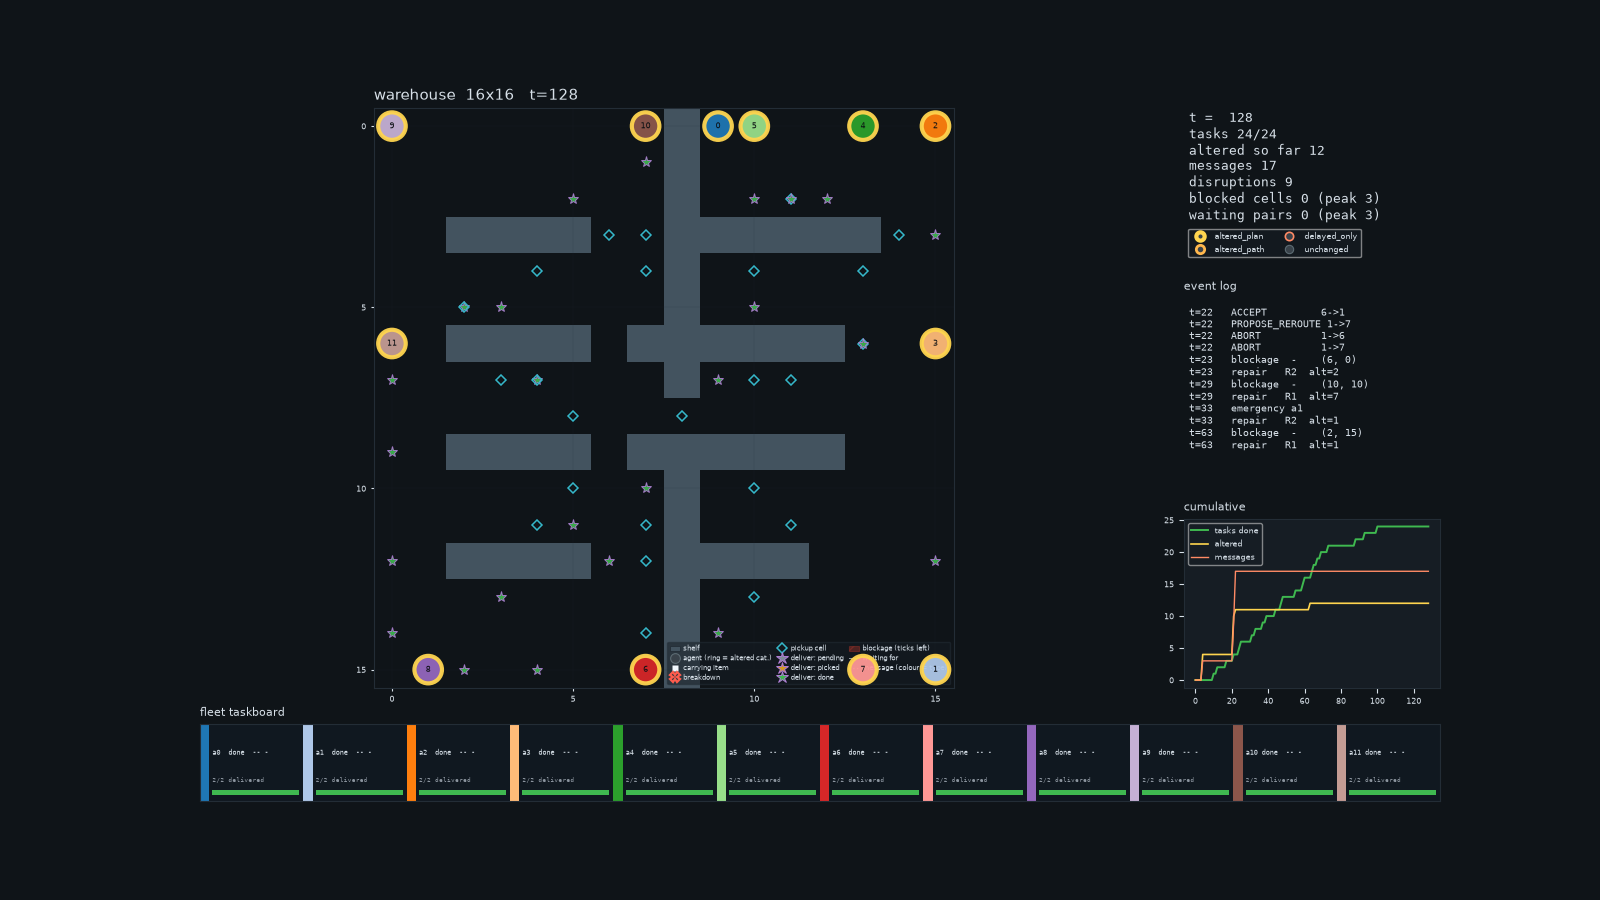
\includegraphics[width=0.66\textwidth]{caseA_final_panel.png}
\caption{The congested shift at its final tick.  The single door of the
closed aisle is the dark gap in the wall, the colours of the robots record
which of them the repair altered, and the counters in the panel are the ones
tabulated above.}
\label{fig:finalpanel}
\end{figure}

The per-event data provide detail that the aggregate table does not.  The
first event ($t=4$, a lane closing on a route) already involves four robots
and three messages, and the accident at $t=22$ is the most costly pass of the
shift, affecting eight of twelve robots and eight of the seventeen messages.

\begin{table}[H]
\centering
\small
\setlength{\tabcolsep}{5pt}
\begin{tabular}{@{}r l c r r r r r r@{}}
\toprule
$t$ & \textbf{event} & \textbf{rung} & \textbf{plan} & \textbf{path} &
\textbf{delayed} & \textbf{naive} & \textbf{delay} & \textbf{msgs}\\
\midrule
4  & blockage           & R2 & 4 & 4 & 0 & 4 & 79 & 3\\
21 & blockage           & R2 & 2 & 2 & 0 & 2 & 13 & 6\\
22 & accident+blockage  & R2 & 8 & 8 & 0 & 8 & 51 & 14\\
21 & conflict           & R2 & 7 & 7 & 0 & 7 & 37 & 17\\
23 & blockage           & R2 & 2 & 2 & 0 & 2 & 10 & 17\\
29 & blockage           & R1 & 7 & 8 & 0 & 8 & 1  & 17\\
33 & emergency          & R2 & 1 & 1 & 0 & 1 & 24 & 17\\
63 & blockage           & R1 & 1 & 1 & 0 & 1 & 2  & 17\\
\bottomrule
\end{tabular}
\caption{The eight repair passes of case study~A, in execution order.
\emph{plan}, \emph{path}, \emph{delayed} and \emph{naive} are the four
altered-agent counts of the pass, \emph{delay} is the pass's added delay in
ticks and \emph{msgs} is the cumulative number of protocol messages.  The
first four passes each end with a negotiated grant (the cumulative message
count rises); the last two are $R_1$ self-reroutes with no messages.}
\label{tab:passesA}
\end{table}
All 24 tasks are delivered and every tick validates.  The repair touched all
twelve robots, through eight separate local passes: six resolved at rung
$R_2$ and two as $R_1$ self-reroutes.  The shift incurs $217$ ticks of delay
in total, $51$ of them from the accident at $t=22$, and a pass takes
$8$--$195$\,ms of CPU.

\subsection{Comparison of repair strategies}

The same nine events are replayed against five strategies on the same
instance: the negotiated repair, a self-only ladder (no reordering of tasks),
the BFS-prioritised baseline, a global re-planning upper bound that replans
\emph{every} robot from its current state at every event, and a no-repair
ablation that freezes the disruptions and repairs nothing.

\begin{table}[H]
\centering
\small
\setlength{\tabcolsep}{5pt}
\begin{tabular}{@{}l l c c c c c l@{}}
\toprule
\textbf{mode} & \textbf{status} & \textbf{tasks} & \textbf{makespan} &
\textbf{repairs} & \textbf{altered} & \textbf{msgs} & \textbf{rungs (counts)}\\
\midrule
negotiate & OK            & 24/24 & 128 & 8  & 12 & 17 & R2$\times$6, R1$\times$2\\
self\_only & OK           & 24/24 & 132 & 7  & 7  & 0  & R2$\times$5, R1, R0\\
bfs       & OK            & 24/24 & 142 & 10 & 12 & 33 & R2$\times$6, R1$\times$2, R4\\
global    & 3 violations  & 21/24 & 128 & 23 & 12 & 0  & R2\_restart$\times$23\\
static (no repair) & 20 violations$^{*}$ & 24/24 & 132 & 0 & 0 & 0 & ---\\
\bottomrule
\end{tabular}
\caption{All four repair modes and the no-repair ablation on the identical
event list of case study~A.  $^{*}$\code{static} is an ablation: repairs are
disabled by design, so its violations represent the cost of \emph{not}
repairing.  ``altered'' is the number of distinct robots whose plan changed
at least once.  The negotiated mode is the only strategy that attains the
best makespan (128), delivers every task, validates every tick and completes
the repair in eight passes.}
\label{tab:compare}
\end{table}

Four observations follow.  First, locality does not reduce solution quality:
the negotiated mode attains the best makespan of every safe mode (128) in
eight passes, so its locality carries no time penalty.  The only mode that
touches fewer robots (self\_only, seven) incurs four additional ticks of
makespan and one extra pass, because it may not reorder tasks.  Second, the
global re-planning bound reduces neither scope nor errors: re-planning all
twelve robots at every event produces 23 restart passes, three validation
violations and an incomplete task set (21/24).  The cause is structural, as a
fleet-wide restart cannot respect the already-executed prefix and therefore
issues reservations that the executed part of the schedule has already
consumed; this provides empirical support for the claim that a local repair
is both cheaper and more correct.  Third, self-only repair is inexpensive but
inflexible: forbidding task reordering keeps the altered set at seven robots
but costs four ticks of makespan and one extra pass, because two events
require goal-level reassignment.  Fourth, communication enables a shorter
makespan: \code{bfs} uses 33 messages and ten passes to finish at 142, and it
is the only mode that performs an $R_4$ hand-off on this instance.
\subsection{Case study B: the corridor choke point}\label{sec:caseB}

The congested warehouse is dense but does not force negotiation: a robot can
usually leave through another gap, so the protocol is an option rather than a
requirement.  The corridor is the opposite case.  An $8\times10$ world is
divided by a wall with a single door at $(3,3)$; robot~0 parks on the door
and robot~1 is locked out of it, and both robots of that pair are inoperative
from early in the run.  No conflict-free hard detour is therefore available,
because any route for robot~1 passes through the door occupied by robot~0,
and the ladder is forced onto the negotiation rungs.

\begin{table}[H]
\centering
\small
\setlength{\tabcolsep}{6pt}
\begin{tabular}{@{}l l@{}}
\toprule
\textbf{Quantity} & \textbf{Value}\\
\midrule
instance          & \code{negotiate}, $8\times10$ corridor, $N=4$, door $(3,3)$\\
tasks delivered   & 3 of 3\\
makespan          & 19 ticks\\
validated safe    & yes\\
repair passes     & 1 (rung $R_2$)\\
robots altered    & 2 (the parked holder and the locked-out robot)\\
protocol messages & 3 (\textsc{Propose\_Reroute}, \textsc{Accept}, \textsc{Commit})\\
panel peaks       & 2 altered agents, 3 messages, 2 disruptions,\\
                  & 0 closed cells, 0 waiting pairs\\
FAILED\_INIT      & 0\\
\bottomrule
\end{tabular}
\caption{Case study B.  One pass, resolved at $R_2$, three messages and two
robots altered, the minimum for a clash that no hard detour can avoid.  The
two zero counters are consistent: the corridor has no closed lane and no
queue, so the counters and the message log measure different quantities and
agree.}
\label{tab:caseB}
\end{table}

The dialogue of the pass has the expected form: the initiator proposes a
reroute over the door, the holder accepts, and the pass commits
(\textsc{Propose\_Reroute}, \textsc{Accept}, \textsc{Commit}), three messages
and one altered pair.  No robot outside the pair is changed, because no other
robot's route crosses the door.

\begin{figure}[H]
\centering
\begin{subfigure}[t]{0.72\textwidth}
  \centering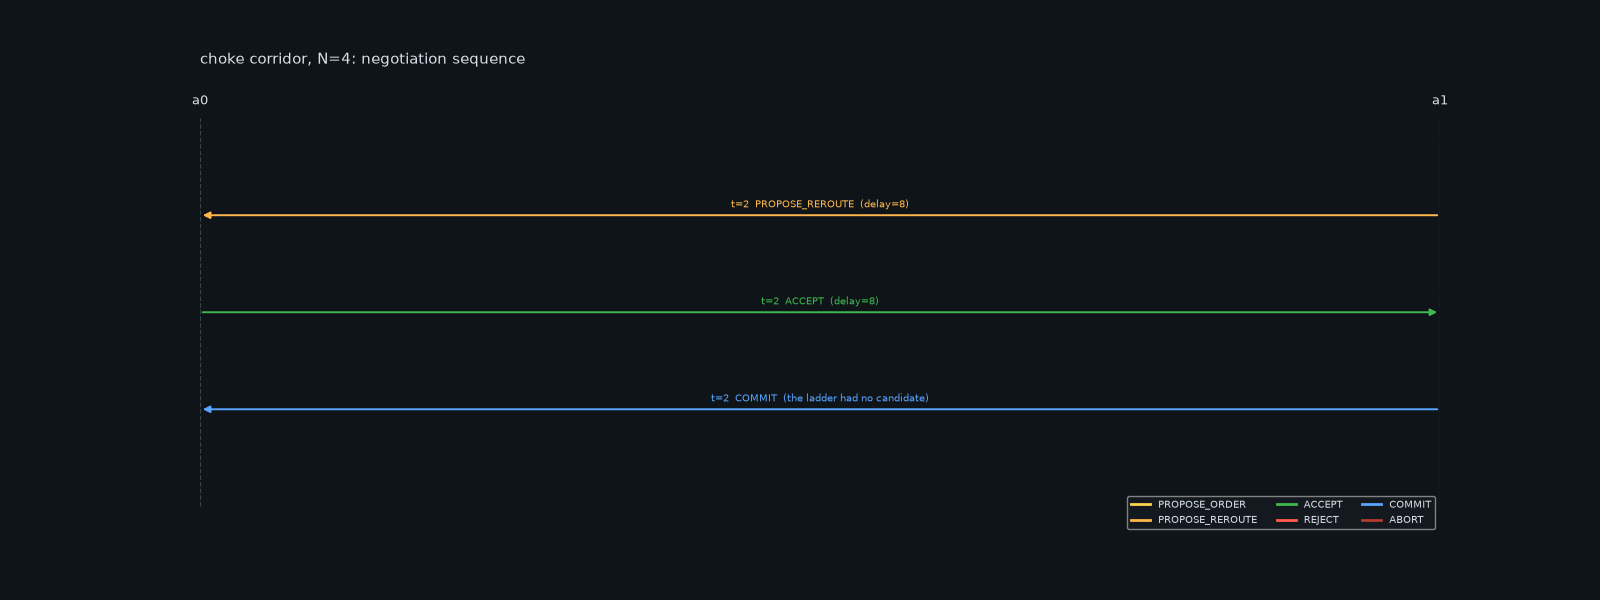
\includegraphics[width=\linewidth]{caseB_sequence.png}
  \vspace{2pt}
  \caption{message-sequence diagram of the pass}
\end{subfigure}

\vspace{4pt}
\begin{subfigure}[t]{0.92\textwidth}
  \centering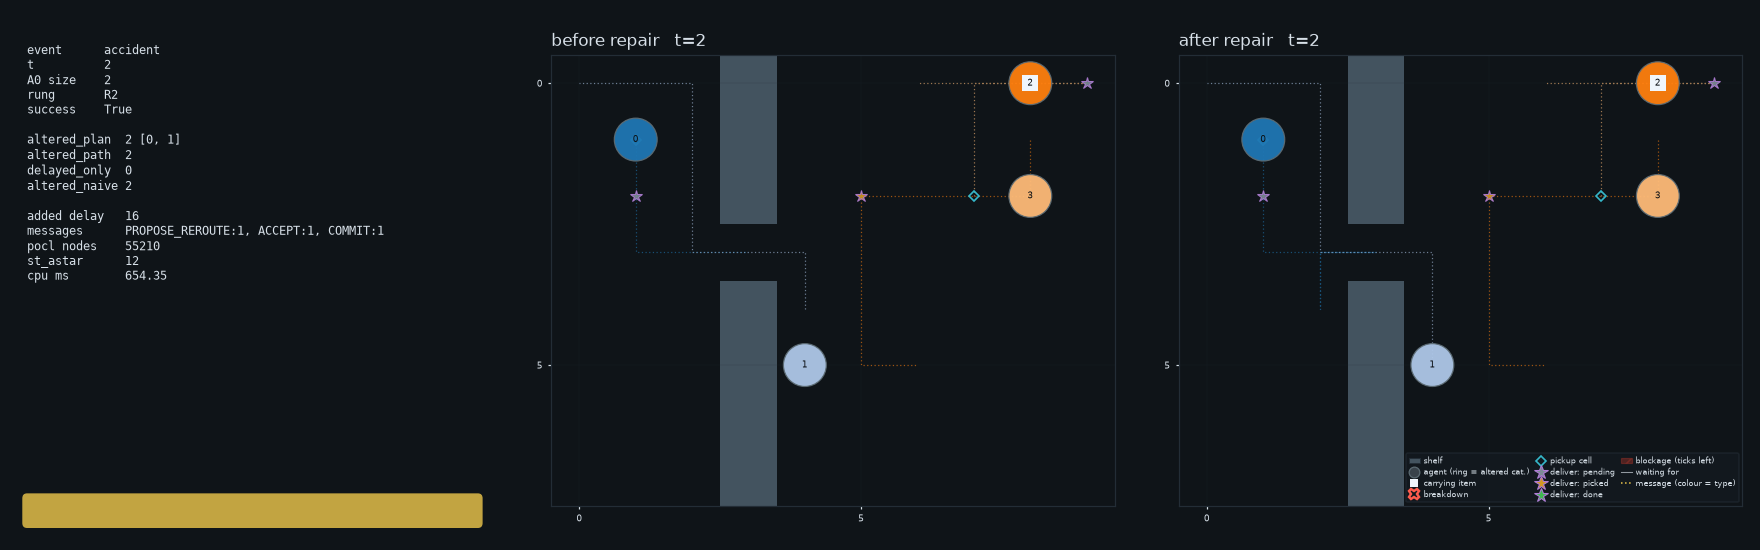
\includegraphics[width=\linewidth]{caseB_repair_card.png}
  \caption{the repair card of the pass ($t=2$, $R_2$, two altered robots)}
\end{subfigure}
\caption{Case study~B in two views: the message-sequence diagram (time on the
vertical axis, the robot pair on the horizontal axis, one arrow per protocol
message with its type and the cell it concerns) and the repair card.  The
arrows describe the repair decision: the initiator asks first, the holder
grants second, and only the committing arrow changes a schedule.}
\label{fig:caseB}
\end{figure}

Comparing the two case studies isolates the role of the protocol.  Of the
eight passes of case~A, four conclude with negotiation (17 messages in
total), two are $R_1$ self-reroutes with no messages, and two are resolved by
a longer detour that requires no negotiation; the ladder communicates only
when the geometry admits no other locally computed option.  In case~B the
same ladder has no such option: one clash, one negotiation, three messages.
The protocol is therefore not a general-purpose scheduler but a mechanism
that converts a locally impossible detour into a two-robot agreement.

\subsection{Parameter sweep}

The two case studies are single instances.  To verify that their results are
not specific to one chosen warehouse, the same pipeline is run over a grid of
instance families: an open $30\times30$ warehouse with $N \in \{5, 10\}$
robots, aisle-closure densities of $0\%$ and $5\%$, ten seeds per cell, three
tasks per robot and the same event generator, giving $40$ families per mode
and $120$ runs in total.  Each run also emits one row per disruption, so the
sweep produces $1361$ disruption records in addition to the $120$ summary
rows.

\begin{table}[H]
\centering
\small
\setlength{\tabcolsep}{5pt}
\begin{tabular}{@{}l c c c c c c c c@{}}
\toprule
\textbf{mode} & \textbf{plan} & \textbf{naive} & \textbf{cost} &
\textbf{makespan} & \textbf{succ.} & \textbf{safe} & \textbf{A$^\ast$} &
\textbf{msgs}\\
\midrule
global    & 5.047 & 5.498 & 1824.5 & 190.8 & 1.000 & 38/40 & 1251.4 & 0.00\\
negotiate & 1.572 & 1.634 & 2083.8 & 221.0 & 0.920 & 40/40 &  100.5 & 0.00\\
self\_only & 1.150 & 1.150 & 2085.7 & 220.9 & 0.931 & 40/40 &   45.9 & 0.00\\
\bottomrule
\end{tabular}
\caption{Per-mode means over the $40$ families of the sweep (three tasks per
robot, $30\times30$).  Columns: the mean \code{altered\_plan} and
\code{altered\_naive} count per event, the sum of costs, the makespan,
\emph{succ.} $=$ the fraction of disruptions repaired within the budget,
\emph{safe} $=$ the families in which \emph{no} tick of the run produced a
validation violation, \emph{A$^\ast$} $=$ the mean number of space-time
searches and \emph{msgs} the mean number of protocol messages.}
\label{tab:sweep}
\end{table}

The sweep yields four results.  First, the locality advantage is substantial:
a negotiated repair alters $1.57$ robots per event on average, against $5.05$
for the global restart; the median instance alters $1.50$, $35$ of the $40$
families remain at or below $2$, and the mean ratio of the global altered-set
size to the local one is $3.29$.  Second, locality is paid for in travel
rather than in correctness: the sum of costs rises from $1825$ to $2084$
($+14\%$) and the makespan from $191$ to $221$, the expected cost of not
re-planning the fleet; however, every negotiated and self-only run is
conflict-free while the global bound is not ($38/40$ families, two runs with
residual conflicts), and the number of space-time searches follows the same
pattern ($100$ for local repair against $1251$ for the restart), so locality
also reduces planner effort.  Third, failures appear as waiting rather than
as collisions: in $8$ of the $40$ negotiated families one robot does not
complete its task within the default retry budget (a mean success rate of
$0.92$, the worst family at $0.50$), and every one of those runs remains
conflict-free; an exhausted ladder keeps the robot waiting ($R_0$ fallback)
and records \code{success = False}, which is the intended failure mode
(slower but not unsafe).  Fourth, the protocol is not used in an open
warehouse: the mean number of messages is $0.00$ in all three modes, because
on a $30\times30$ grid with sparse blockages either the hard detour of $R_1$
or the longer detour of $R_2$ is always available.  This is the reason both
case studies use a constrained instance.
\begin{figure}[H]
\centering
\begin{subfigure}[t]{0.47\textwidth}
  \centering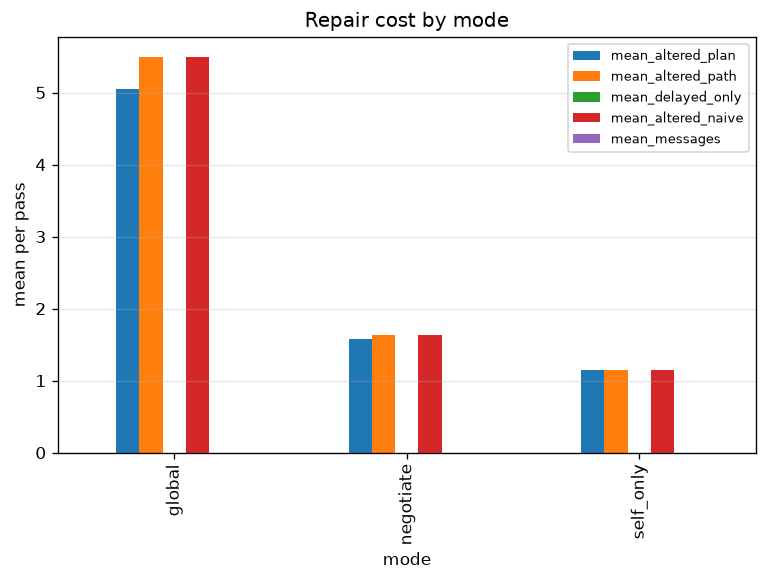
\includegraphics[width=\linewidth]{sweep_mode_bars.png}
  \caption{altered robots per event, by mode}\label{fig:sw_bars}
\end{subfigure}\hfill
\begin{subfigure}[t]{0.47\textwidth}
  \centering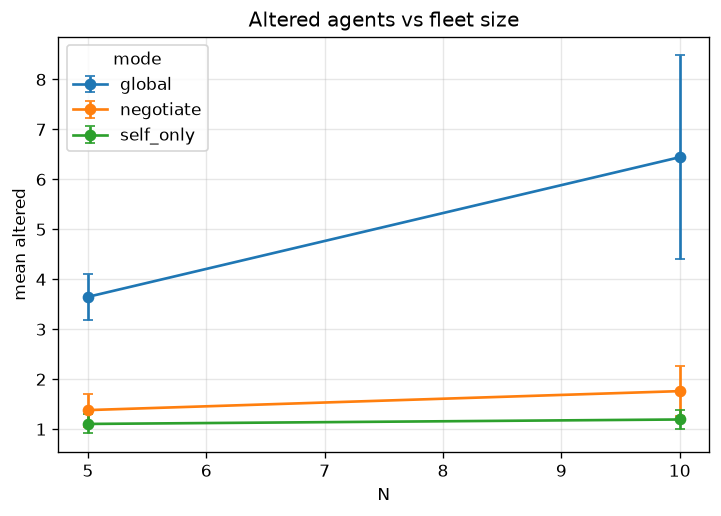
\includegraphics[width=\linewidth]{sweep_altered_vs_N.png}
  \caption{altered robots as a function of $N$}\label{fig:sw_altered}
\end{subfigure}

\vspace{4pt}
\begin{subfigure}[t]{0.47\textwidth}
  \centering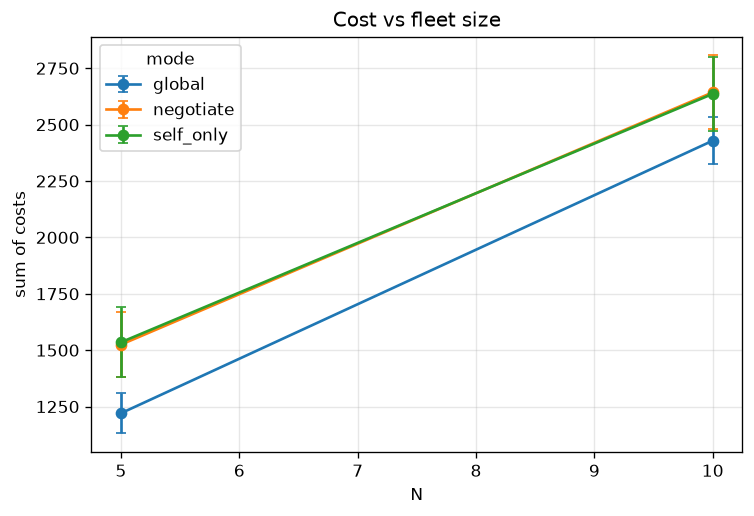
\includegraphics[width=\linewidth]{sweep_cost_vs_N.png}
  \caption{sum of costs as a function of $N$}\label{fig:sw_cost}
\end{subfigure}\hfill
\begin{subfigure}[t]{0.47\textwidth}
  \centering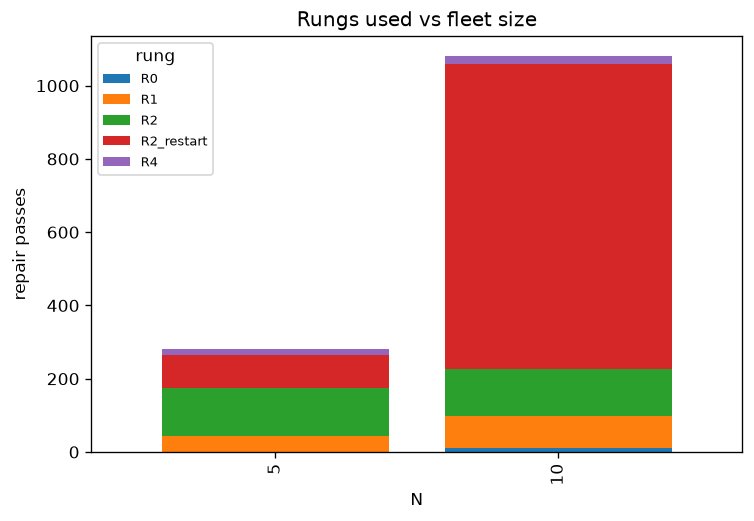
\includegraphics[width=\linewidth]{sweep_rung_stack_vs_N.png}
  \caption{which rungs resolve the passes}\label{fig:sw_rungs}
\end{subfigure}
\caption{The sweep in four views.  The gap between the global restart and the
local modes in (a)--(b) is the locality result; (c) shows that the cost of
locality is a mild increase in travel that grows with $N$; and (d) shows which
rung resolved each pass.  The two local modes remain on the low rungs, while
every pass of the global baseline is a full restart, which accounts for its
larger bar.  The artefacts also contain a cost heat-map over the
$(N, \text{density})$ grid and a plot of the four altered-agent definitions
side by side.}
\label{fig:sweep}
\end{figure}

% =====================================================================
\subsection{Fleet-size and blockage-density scaling}\label{sec:scaling}

The grid of the previous subsection varies only $N \in \{5,10\}$ at two
densities, so it cannot separate fleet size from instance size, and its largest
fleet is far below the $12$-robot case study.  The sweep is therefore extended
along two independent axes on the same open $30\times30$ warehouse, with the
same three tasks per robot, the same event generator and ten seeds per cell:
the fleet grows over $N \in \{5,10,20,30\}$ at a fixed $5\%$ blockage density
and, independently, at $N=20$ the density grows over $\{0,2,5,10\}\%$.  The two
sweeps share the $(N{=}20, 5\%)$ cell, so they comprise $63$ instance families
and $189$ runs; table~\ref{tab:scaling} reports the per-cell means.

\begin{table}[H]
\centering
\small
\setlength{\tabcolsep}{4pt}
\begin{tabular}{@{}l r c r r r c r@{}}
\toprule
\textbf{mode} & \textbf{$N$} & \textbf{$n$} & \textbf{altered} &
\textbf{sum of costs} & \textbf{makespan} & \textbf{succ.} &
\textbf{A$^\ast$}\\
\midrule
\multicolumn{8}{@{}l}{\emph{(a) fleet size, density fixed at $5\%$}}\\
\midrule
negotiate & 5  & 10 & 1.43  & 1532.7 & 227.9 & 0.958 &    93.5\\
negotiate & 10 & 10 & 1.83  & 2710.9 & 228.1 & 0.958 &   163.0\\
negotiate & 20 &  9 & 2.13  & 5128.1 & 214.0 & 0.981 &  3567.0\\
negotiate & 30 &  8 & 3.35  & 7664.4 & 216.2 & 0.977 &  3102.8\\
self\_only & 5  & 10 & 1.10 & 1532.2 & 227.7 & 0.958 &    42.6\\
self\_only & 10 & 10 & 1.19 & 2707.7 & 227.8 & 0.959 &    68.8\\
self\_only & 20 &  9 & 1.21 & 5097.2 & 213.1 & 0.990 &   342.1\\
self\_only & 30 &  8 & 1.31 & 7550.9 & 212.9 & 0.988 &   314.4\\
global & 5  & 10 & 3.56 & 1225.3 & 187.9 & 1.000 &   158.4\\
global & 10 & 10 & 5.70 & 2451.4 & 195.7 & 1.000 &  4474.4\\
global & 20 &  9 & 14.91 & 5109.1 & 203.7 & 1.000 &  1200.7\\
global & 30 &  8 & 18.58 & 7893.6 & 212.2 & 0.947 &  8167.2\\
\midrule
\multicolumn{8}{@{}l}{\emph{(b) blockage density, $N$ fixed at $20$}}\\
\midrule
negotiate & 0    & 10 & 2.85 & 5082.8 & 219.1 & 0.983 &   145.3\\
negotiate & 0.02 &  9 & 2.64 & 5070.6 & 212.2 & 0.966 &   181.8\\
negotiate & 0.05 &  9 & 2.13 & 5128.1 & 214.0 & 0.981 &  3567.0\\
negotiate & 0.10 &  6 & 2.89 & 5122.2 & 211.0 & 0.982 &   442.2\\
self\_only & 0    & 10 & 1.32 & 5085.6 & 222.4 & 0.983 &    48.0\\
self\_only & 0.02 &  9 & 1.27 & 5053.0 & 212.7 & 0.968 &    55.4\\
self\_only & 0.05 &  9 & 1.21 & 5097.2 & 213.1 & 0.990 &   342.1\\
self\_only & 0.10 &  6 & 1.29 & 5047.0 & 212.0 & 0.984 &   137.2\\
global & 0    & 10 & 15.93 & 4968.2 & 197.8 & 1.000 &   496.2\\
global & 0.02 &  9 & 13.26 & 4982.1 & 200.1 & 1.000 &  2110.4\\
global & 0.05 &  9 & 14.91 & 5109.1 & 203.7 & 1.000 &  1200.7\\
global & 0.10 &  6 & 12.89 & 5316.3 & 204.8 & 1.000 & 11157.3\\
\bottomrule
\end{tabular}
\caption{Two scaling sweeps on the open $30\times30$ warehouse.  Columns are as
in table~\ref{tab:sweep}, with \emph{altered} the mean \code{altered\_plan}
count per event and $n$ the number of seeds that completed inside the compute
budget.  Cells with $n<3$ are omitted, which is why the axes stop at $N=30$ and
$10\%$ density: the mean repair pass of a large, densely blocked instance grows
with $N^{2}$ and with the blockage count, and the remaining cells did not
finish in time to be reported.}
\label{tab:scaling}
\end{table}

Three conclusions follow.  \emph{(i) The locality advantage grows with the
fleet.}  The global restart re-plans $0.62N$ robots per event --- $3.56$ at
$N=5$ and $18.58$ at $N=30$ --- whereas a negotiated repair alters
$1.43 \rightarrow 3.35$ robots and a self-only reroute $1.10 \rightarrow 1.31$;
the ratio of the global altered-set size to the negotiated one therefore rises
from $2.5$ at $N=5$ to $5.5$ at $N=30$, and reaches $14$ against self-only.
\emph{(ii) The travel cost of locality is recovered at scale.}  At $N=5$ the
restart is both the cheapest method ($1225$ against $1533$, i.e.\ $-20\%$) and
$40$ ticks faster; by $N=30$ the ordering has reversed, the local modes are the
cheaper ones ($7664$ and $7551$ against $7894$) and the makespan gap has
collapsed to $4$ ticks.  The reason is structural: a restart re-plans the entire
fleet at every event, so its aggregate travel grows with $N$, while a repair
re-plans one robot regardless of how large the fleet is.  \emph{(iii) The
restart also loses its safety margin.}  It is the only mode with residual
validation failures, and its success rate falls to $0.947$ at $N=30$ (one family
in eight), against $0.977$ negotiated and $0.988$ self-only, while its planner
effort explodes --- $8167$ space-time searches at $N=30$, $2.6\times$ the
negotiated count and $26\times$ the self-only count.

The density axis behaves differently: it is almost neutral.  From $0\%$ to $10\%$
closed lanes the negotiated repair alters $2.85 \rightarrow 2.89$ robots per
event and its sum of costs moves by less than $1\%$; self-only alters
$1.32 \rightarrow 1.29$.  The altered set of the global restart is nearly as
neutral ($15.9 \rightarrow 12.9$), but its \emph{effort} is not: its space-time
searches grow from $496$ to $11157$, a factor of $22$, because every additional
closed lane lengthens the shortest paths that the full restart recomputes for
every robot, whereas the local modes keep searching inside a two-robot
neighbourhood.  Locality is thus invariant to how congested the warehouse is,
and increasingly valuable as the fleet grows; the two effects compound, since a
large fleet in a densely blocked warehouse is precisely the regime in which the
restart is slowest to compute and least safe.

As in the smaller grid, no cell of either sweep exchanges a single protocol
message (the mean is $0.00$ in all $24$ cells): with three tasks per robot on an
open grid, either the hard detour of $R_1$ or the longer detour of $R_2$ is
always available, which is why both case studies again use constrained
instances.  The two sweeps therefore reproduce the central result of the
previous subsection --- a local mode alters an order of magnitude fewer robots
than a global restart --- and show that the gap widens rather than closes as the
fleet scales.

\begin{figure}[H]
\centering
\begin{subfigure}[t]{0.48\textwidth}
  \centering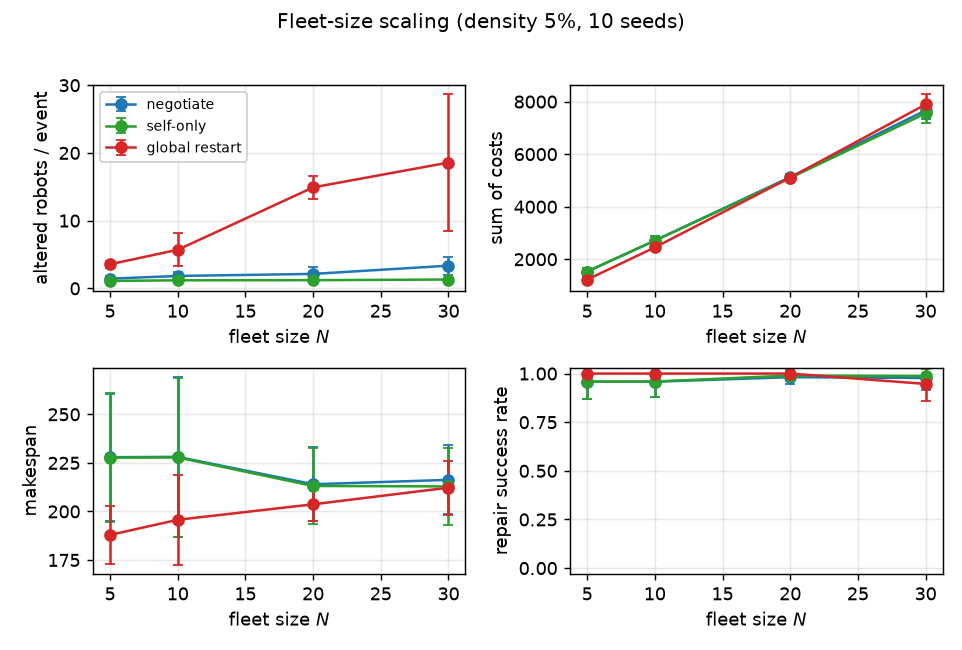
\includegraphics[width=\linewidth]{scaling_vs_N.png}
  \caption{fleet size $N$ at $5\%$ density}\label{fig:sc_n}
\end{subfigure}\hfill
\begin{subfigure}[t]{0.48\textwidth}
  \centering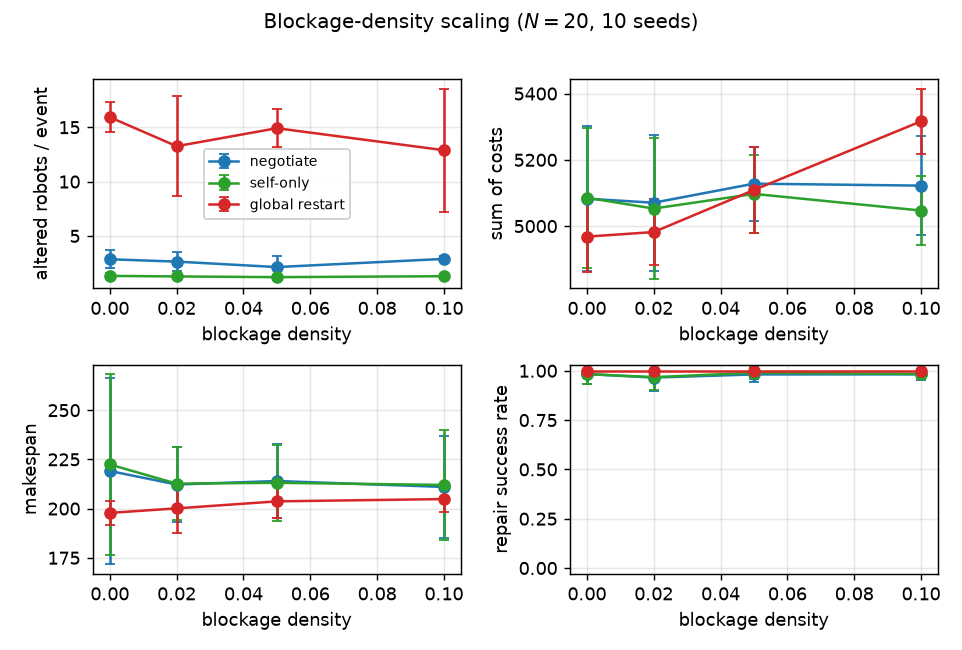
\includegraphics[width=\linewidth]{scaling_vs_density.png}
  \caption{blockage density at $N=20$}\label{fig:sc_d}
\end{subfigure}
\caption{The two scaling sweeps, each in four views (altered robots per event,
sum of costs, makespan and repair success rate).  In (a) the global restart's
altered set and travel cost grow with the fleet, and by $N=30$ it is both the
most expensive and the only mode with residual failures, while the two local
modes stay near one to three robots per event; in (b) all three modes are flat
in blockage density, because density lengthens the searches that the restart
must repeat rather than the number of robots a repair touches.  Whiskers are
$\pm1$ standard deviation over the seeds of the cell and the success-rate panels
are pinned to $[-0.03,1.03]$.}
\label{fig:scaling}
\end{figure}

% =====================================================================
\section{Discussion}\label{sec:discussion}
% =====================================================================

\textbf{Consequences of the partial-order representation.}  The measurements
support the design hypothesis in a specific, checkable form: the difference
between the plan measure and the naive trace measure is exactly the set of
robots whose \emph{timing} changed but whose \emph{plan} did not, and this
set is non-empty because the plan is a partial order.  A timetable
representation has no such set: whenever a robot waits, its plan changes, and
re-scheduling is indistinguishable from re-planning.  The $t=29$ row of
Table~\ref{tab:passesA} (plan $7$ against path $8$ for one tick of added
delay) is the smallest instance of this effect, and the sweep table shows the
same ordering at scale ($1.572$ against $1.634$).

\textbf{Failure modes.}  Three failure modes are reported.  An \emph{exhausted
ladder} ($8$ of $40$ negotiated families) leaves one robot unfinished but the
run conflict-free: a local repair cannot complete every task under every
budget, but it does not produce unsafe schedules.  A \emph{disconnected map},
that is, a disruption that permanently removes the last edge between two
halves of the warehouse, cannot be repaired locally: the affected task is
unreachable, and the two available responses are to transfer the goal to a
robot on the other side (rung $R_4$, exercised by the BFS baseline in
Table~\ref{tab:compare}) or to report failure; both are implemented.  Finally,
a \emph{global restart does not constitute a safe upper bound}: the strategy
with the most freedom produces the only violations and the only incomplete
task set on the congested instance, because once a plan is executing, a
fleet-wide restart issues reservations that the executed prefix has already
consumed.

\textbf{Limitations.}  The evaluation has three limitations.  First, the
sweeps use a fixed grid of $N \in \{5, 10\}$ at two densities: the trend is
clear, but the $N$ range is small and the largest instance is far smaller
than a real warehouse fleet.  Second, \code{cpu\_ms} is wall-clock time and
is therefore not reproducible; every other column of every table is.  Third,
the negotiation is evaluated with one fixed budget (\code{max\_depth},
\code{delay\_threshold}, \code{beta\_alter}); the sensitivity of the message
count and of the altered sets to these parameters is a natural next
experiment, and the code already exposes standalone sweeps for the
communication radius and for the POP node budget.
% =====================================================================
\section{Reproducing the results}\label{sec:run}
% =====================================================================

\textbf{Environment.}  Python 3.10 or newer (the results here were produced
with 3.12), with NumPy, pandas and Matplotlib; \code{pytest} for the test
suite and \code{ffmpeg} optionally for MP4 export.  Nothing in the pipeline
needs a GPU and no step needs network access.  The sources, the test suite and
every artefact referenced in this report live at
\url{https://github.com/aaditya-biswas/AS_Assignment}.

\textbf{Determinism.}  There is a single seeded random stream per run, every
set or dictionary iteration that feeds a decision is sorted, and the whole
suite is meant to be run with \code{PYTHONHASHSEED=0}.  Every table in this
report is reproduced exactly by the commands below; the only column that is
not reproducible is the wall-clock \code{cpu\_ms} of a repair pass.

\begin{lstlisting}[style=shell]
# 1. the congested shift of case study A (12 robots, 16x16, 9 events)
python run_demo.py

# 2. the same shift, every repair strategy on the identical event list
python run_demo.py --compare

# 3. the same shift with the figures of this report
python run_demo.py --compare --viz --outdir outputs

# 4. the corridor of case study B (the protocol is forced to speak)
python run_demo.py --choke --compare --viz --outdir outputs/choke

# 5. the parameter sweep (results.csv + the plots of the sweep figure)
python experiments.py --sweep grid --seeds 10 --plots

# 6. the test suite
PYTHONHASHSEED=0 python -m pytest -q
\end{lstlisting}

The test suite contains more than 110 tests.  The tests most relevant to the
claims of this report are the multi-seed safety tests
(\code{test\_peg\_sim.py}, \code{test\_planner.py}), which assert over many
seeds that a completed run has no validation violations, that every task is
delivered and that every robot ends parked on its own cell, the invariant
that a repair must preserve.

\textbf{Animated artefacts.}  Each mode is also exported as an animation
(an \code{animation.gif} in each mode's output directory), one frame per tick
at a playback rate chosen so that the protocol dialogue can be read while it
plays:
\code{negotiate} is the congested shift analysed in Tables~\ref{tab:caseA}
and~\ref{tab:passesA}, \code{self\_only} the same shift without task
reordering, \code{bfs} the baseline with the only $R_4$ hand-off of the
instance, \code{global} the restart that produces the violations, and
\code{static} the no-repair ablation.  The runs are also exported as still
frames (\code{caseA\_shot\_t0}, $t=22$, $t=128$).
% =====================================================================
\section{Conclusion}
% =====================================================================

A planner and simulator for a multi-robot warehouse were built and used to
evaluate one hypothesis: that a disruption can be repaired \emph{locally}
when the plan is stored as a partial order, and that where a local detour is
geometrically impossible a short negotiation between the robots holding the
contested cells supplies the missing freedom.  The evidence is consistent
across two instances and a $120$-run sweep, where a negotiated repair alters
about one third as many robots per event as a fleet-wide restart, incurs a
small fraction of the search effort, and never produces a validation
violation, and on the congested instance it is the only strategy that
completes the task set.  The global restart, which is unconstrained by
locality, ends with violations and three undelivered tasks because it cannot
respect the part of the plan that has already executed.  The two case studies
show the protocol in both regimes: no messages when the geometry admits a
detour, and three messages when it does not.

The next steps follow from the limitations: increase $N$ and the load so that
the ladder's failure mode is common rather than rare, sweep the negotiation
budget and the communication radius, and extend the repair to negotiate about
\emph{goals} as well as about cells, since a task hand-off agreed between two
robots is the natural generalisation of the $R_4$ rung.

% =====================================================================
\begin{thebibliography}{9}
% =====================================================================

\bibitem{mcallester91} D. McAllester and D. Rosenblitt.
  \emph{Systematic Nonlinear Planning.}  AAAI-91, 1991.

\bibitem{ucpop} J. Penberthy and D. Weld.
  \emph{UCPOP: A Sound, Complete, Partial Order Planner for ADL.}
  KR-92, 1992.

\bibitem{kambhampati92} S. Kambhampati and J. Hendler.
  \emph{A Validation-Structure-Based Theory of Plan Modification and Reuse.}
  Artificial Intelligence 55(2--3), 1992.

\bibitem{silver05} D. Silver.
  \emph{Cooperative Pathfinding.}  AIIDE-05, 2005.

\bibitem{cbs} G. Sharon, R. Stern, A. Felner and N. Sturtevant.
  \emph{Conflict-Based Search for Optimal Multi-Agent Pathfinding.}
  Artificial Intelligence 219, 2015.

\bibitem{lifelong} H. Ma, J. Li, S. Koenig and T. K. S. Kumar.
  \emph{Lifelong Multi-Agent Path Finding for Online Pickup and Delivery
  Tasks.}  AAMAS-17, 2017.

\bibitem{survey} R. Stern, N. Sturtevant, A. Felner, S. Koenig, H. Ma,
  T. Walker, J. Li, D. Atzmon, L. Cohen, T. Kumar, E. Boyarski and R. Bart\'ak.
  \emph{Multi-Agent Pathfinding: Definitions, Variants, and Benchmarks.}
  SoCS-19, 2019.

\bibitem{kiva} P. Wurman, R. D'Andrea and M. Mountz.
  \emph{Coordinating Hundreds of Cooperative, Autonomous Vehicles in
  Warehouses.}  AI Magazine 29(1), 2008.

\end{thebibliography}

\end{document}
